\documentclass[11pt]{article}

\usepackage[a4paper,margin=1in]{geometry}
\usepackage[T1]{fontenc}
\usepackage[utf8]{inputenc}
\usepackage{lmodern}
\usepackage{microtype}
\usepackage{amsmath,amssymb,amsthm,mathtools,bm}
\usepackage{booktabs}
\usepackage{enumitem}
\usepackage{natbib}
\usepackage{hyperref}
\usepackage{setspace}
\usepackage{graphicx}
\usepackage{array}
\usepackage{float}
\usepackage{caption}

\hypersetup{colorlinks=true,citecolor=blue,linkcolor=blue,urlcolor=blue}
\setstretch{1.06}
\setlength{\emergencystretch}{3em}
\graphicspath{{figures/}}

\newtheorem{assumption}{Assumption}
\newtheorem{proposition}{Proposition}
\newtheorem{remark}{Remark}
\newtheorem{definition}{Definition}

\newcommand{\E}{\mathbb{E}}
\newcommand{\Prob}{\mathbb{P}}
\newcommand{\1}{\mathbf{1}}
\newcommand{\R}{\mathbb{R}}
\newcommand{\Aset}{\mathcal{A}}
\newcommand{\Vset}{\mathcal{V}}
\newcommand{\dd}{\,\mathrm{d}}

\title{\bfseries Endogenous Credibility in Social Learning}
\author{Gabriel Bontemps \and Abhishek Banerjee}
\date{June 2026}

\begin{document}
\maketitle

\begin{abstract}
\noindent
Connected groups sometimes learn faster than isolated individuals, yet
sometimes converge confidently on the wrong answer. We argue that part of the
explanation is that social signals are not neutral: they are weighted by a
\emph{credibility} that is generated endogenously by the decision process
itself. We develop an agent-based model in which each agent is a reinforcement
learner whose binary choices arise from a drift--diffusion process. The same
within-trial process produces an endogenous confidence signal, and confidence
acts as a credibility weight in two distinct social channels: an
\emph{anticipatory} channel, through which neighbours' past confidence-weighted
actions enter subjective value before choice, and a \emph{retrospective}
channel, through which neighbours' observed outcomes modulate value revision
after choice. Agents are embedded in community-structured networks; under
balanced block weights the anticipatory social field admits an exact quotient
representation over communities (for any number of communities). We implement the
model, verify it against a ten-point test contract, and study it by Monte Carlo
simulation in two-community societies and a four-community modular extension. The
simulations identify four interpretable regimes
--- efficient consensus, wrong consensus, polarisation and unresolved learning
--- and show that connectivity is \emph{non-monotone}: moderate
credibility-weighted transmission corrects error and accelerates consensus,
whereas strong transmission amplifies early overconfident mistakes. Whether the
distortion takes the form of society-wide wrong consensus or of persistent
between-community divergence is governed by cross-community permeability.
Decisive ablations, identified by common random numbers, show that the
wrong-consensus regime is not a generic consequence of social learning: at the
contested operating point, removing the anticipatory channel, the retrospective
channel, or the decision-time dependence of confidence eliminates it; removing
the credibility weighting weakens but does not eliminate it; and constant
learning rates intensify it. We report Wilson and bootstrap intervals throughout
and confirm the phase structure against threshold, horizon, reward-gap,
initial-condition, grid-resolution and random-graph perturbations. The
contribution is to show that connectivity is conditionally beneficial, and that
its sign depends on whether credibility tracks accuracy or amplifies early
error. A complete replication package reproduces every figure and table.
\end{abstract}

\noindent\textbf{Keywords:} social learning; credibility; confidence;
drift--diffusion model; reinforcement learning; community networks; agent-based
simulation; quotient aggregation; Monte Carlo.

\section{Introduction}

A long tradition in the social and economic sciences holds that connecting
learners is broadly beneficial: pooling dispersed information should, on
average, move groups towards better collective beliefs
\citep{DeGroot1974,GolubJackson2010}. Yet the same literature documents the
opposite outcome just as often. Informational cascades can lock groups onto
incorrect actions \citep{BikhchandaniHirshleiferWelch1992}, crowds can be wise
or mad depending on subtle features of how information is shared
\citep{TumpPleskacKurvers2020}, and reward-like social feedback can entrench
polarisation even on fixed networks \citep{HornBanischBatzdorferReitenbachSartoriSchwabeMas2026}.
The unresolved question is therefore not \emph{whether} connectivity helps, but
\emph{when}: under what conditions does adding social links correct individual
error, and under what conditions does it amplify it into confident collective
mistakes or persistent divergence between groups? Our central hypothesis is that
the answer is decided by an endogenous, socially transmitted variable --- the
\emph{credibility} of a signal, generated by the sender's own decision confidence
--- so that connectivity corrects error when credibility tracks accuracy and
amplifies it when credibility tracks early, possibly mistaken, conviction
(Figure~\ref{fig:mechanism} sketches the mechanism).

We propose that an important part of the answer lies in what is actually
transmitted. Agents rarely exchange bare actions or unweighted observations.
They transmit actions and outcomes that arrive marked by a sense of how
\emph{credible} they are, and that credibility is not exogenous: it is generated
by the very process that produced the action. We formalise this as
\emph{endogenous credibility}. Confidence is produced by an agent's own
decision process; once it is socially interpreted as credibility, it weights how
strongly a neighbour's behaviour influences others. Because confidence can
attach to correct \emph{or} to incorrect early choices, the same network links
can transmit correction or amplify error. Connectivity is then no longer
uniformly beneficial: its effect depends on whether the circulating credibility
tracks accuracy or tracks early, possibly mistaken, conviction. Its sign is set
by the credibility-generating process behind transmitted behaviour, not by
connection itself.

The model makes this precise with deliberately minimal behavioural machinery.
Each agent carries latent action values that are updated from reward prediction
errors \citep{SuttonBarto2018,DayanDaw2008}. Choices are not produced by a
static policy but by a drift--diffusion process, so that action, decision time
and confidence are jointly determined by the strength of accumulated evidence
\citep{Ratcliff1978,RatcliffSmithBrownMcKoon2016}. Confidence is read out from
that same process \citep{KianiShadlen2009,Drugowitsch2019}. Social influence
operates through two channels that we keep strictly separate: an anticipatory
channel that enters subjective value before the decision, and a retrospective
channel that enters value revision after the outcome is observed. Agents live in
modular networks whose community structure is summarised by a row-stochastic
coupling matrix.

This is an agent-based computational social simulation in the sense
emphasised by recent work in this journal: interactions and aggregates emerge
from explicit behavioural rules rather than being imposed as exogenous
summaries \citep{StoneKunasekaranPoulosMacIntyreHeslop2026}, the design is
documented following the ODD protocol and its decision-oriented extension
\citep{GrimmBergerDeAngelisPolhillGiskeRailsback2010,Grimm2020,MullerBohmeFrankGrabnitzMuller2013},
and the baseline is kept narrow so that its parameters remain identifiable and
its observables remain informative \citep{OlukanWardMallesonGe2026,Carrella2021,McCullochGeWardHeppenstallPolhillMalleson2022}.
The model is implemented, verified against an explicit test contract, and
studied by Monte Carlo simulation; a replication package regenerates every
result.

\paragraph{Contributions.}
The novelty is not the ingredients --- reinforcement learning, drift--diffusion
choice, confidence, and social learning are each established --- but their
coupling: confidence is generated by the \emph{same} decision process that
produces the action, it regulates \emph{both} private and social learning, and
credibility is not a fixed edge weight but an \emph{emergent} property that is
produced by neighbours' decisions and propagates through the network. Concretely,
the paper makes five contributions.
\begin{enumerate}[label=(\roman*),leftmargin=2.4em,itemsep=1pt]
\item It introduces an agent-based model in which confidence is generated by a
process-based choice rule rather than assigned exogenously, and is transmitted
socially as credibility.
\item It distinguishes anticipatory social influence from retrospective social
learning and keeps the two channels separate in prose, equations, code and
ablations.
\item It embeds agents in modular networks and proves that, under balanced
block weights, the anticipatory social field admits an \emph{exact} quotient
representation over communities.
\item Using simulation, it identifies when connectivity corrects error, when it
amplifies early overconfident mistakes into wrong consensus, and when it
produces between-community polarisation, mapping these regimes in a
connectivity phase diagram.
\item It validates the community-level quotient description against the full
agent-level model and delimits where the reduction is faithful.
\end{enumerate}

\section{Background and positioning}
\label{sec:background}

\paragraph{Social learning, herding and networked learning.}
The primary anchor is the literature on collective learning and opinion
formation in networks \citep{GolubSadler2016}. Classical models of consensus and
naive learning explain when decentralised updating aggregates information
efficiently \citep{DeGroot1974,FriedkinJohnsen1990,GolubJackson2010}, and
continuous-opinion and bounded-confidence models explain when interaction yields
consensus, clustering or persistent disagreement
\citep{DeffuantNeauAmblardWeisbuch2000,HegselmannKrause2002,FlacheMasFelicianiChattoeBrownDeffuantHuetLorenz2017}.
The herding and cascade literature explains how rational or boundedly rational
agents can lock onto incorrect actions when they over-weight others' behaviour
relative to their own signal
\citep{Banerjee1992,BikhchandaniHirshleiferWelch1992,TumpPleskacKurvers2020}.
Cooperative and networked multi-armed bandit models study the same tension
between social acceleration and distortion in an explicit reward-learning
setting, including on block-structured graphs
\citep{LandgrenSrivastavaLeonard2021,XuShanGhaffariWangLiuHajiesmaili2025}, and
reward-like social feedback can drive polarisation directly even on fixed
networks \citep{BanischOlbrich2019,HornBanischBatzdorferReitenbachSartoriSchwabeMas2026}.
Our model contributes a mechanism to this tradition: the weight an agent places
on a neighbour is not fixed but is an endogenous credibility produced by that
neighbour's own decision process.

\paragraph{What the model changes relative to adjacent traditions.}
Table~\ref{tab:comparison} positions the model. Relative to DeGroot and
bounded-confidence opinion models, agents do not update opinions by weighted
averaging alone: they learn from stochastic rewards, choose through a process
model, and transmit confidence-marked actions and outcomes. Relative to herding
and cascade models, the credibility attached to social information is not
exogenously given but generated by the neighbour's own decision process.
Relative to cooperative bandit models, the model separates anticipatory
influence on choice from retrospective influence on value revision. Relative to
polarisation ABMs, modular divergence arises from the interaction between
confidence-weighted transmission and reward learning rather than from fixed
homophily or ideological repulsion alone; and relative to
reinforcement-learning drift--diffusion (RLDDM) accounts of individual choice,
the novelty is the social transmission of endogenous credibility on a network.

\begin{table}[t]\centering\small
\caption{Positioning relative to adjacent model families.}
\label{tab:comparison}
\begin{tabular}{p{3.1cm}p{3.2cm}p{2.9cm}p{3.4cm}}
\toprule
Tradition & Typical mechanism & Exogenous element & What this paper changes \\
\midrule
DeGroot / consensus & weighted opinion averaging & weights, signals & confidence generated by the choice process \\
Herding / cascades & action inference & reliability of social signal & credibility is endogenous \\
Cooperative bandits & reward learning across agents & communication weight & two distinct social channels \\
Polarisation ABMs & homophily / social feedback & confidence usually absent & confidence-driven amplification \\
RLDDM (individual) & value-based diffusion choice & no social network & social transmission of credibility \\
\bottomrule
\end{tabular}
\end{table}

\paragraph{Agent-based social simulation and documentation.}
Methodologically the paper follows current practice in computational social
simulation. A recurring theme is that the structures of interest should emerge
from explicit mechanisms rather than be imposed as aggregates
\citep{StoneKunasekaranPoulosMacIntyreHeslop2026}, and that model purpose,
design concepts and implementation should be documented separately
\citep{GrimmBergerDeAngelisPolhillGiskeRailsback2010,Grimm2020,MullerBohmeFrankGrabnitzMuller2013}.
A second theme is discipline about heterogeneity, calibration and observables:
descriptive richness can degrade identifiability if introduced faster than the
inferential apparatus that supports it
\citep{OlukanWardMallesonGe2026,WindrumFagioloMoneta2007,Carrella2021,McCullochGeWardHeppenstallPolhillMalleson2022,PolhillHareBauermannAnzolaPalmerSaltAntosz2021}.
We therefore begin with a homogeneous two-community baseline and add structure
only after the mechanism is isolated. Update scheduling is treated as a
modelling decision rather than an implementation detail, since activation
regimes can alter dynamics
\citep{Axtell2000,CaronLormierHumphryBohanHawesThorbek2008,WeimerMillerHillHodson2019};
we fix synchronous trial timing with a simultaneous post-outcome update. We
also represent modular structure through interpretable community-coupling
parameters rather than an arbitrary graph family, in the spirit of stratified
and block-structured network models
\citep{GoncalvesFierensRego2026,LeeWilkinson2019,Peixoto2014}.

\paragraph{Computational models of social cognition and reinforcement learning.}
Contemporary computational accounts treat social learning with the same
primitives as non-social value learning --- value, prediction error,
uncertainty and learning rate
\citep{RuffFehr2014,LockwoodKleinFlugge2021}. This licenses our decision to let
social information enter the same latent-value machinery as private reward, and
to allow learning rates that depend on confidence rather than being globally
fixed \citep{WangVeismannBanerjeePleger2023}. In this reading the retrospective
channel is an \emph{other-referenced} prediction error, the social counterpart of
the self-referenced reward prediction error, consistent with evidence that social
and non-social learning share prediction-error machinery in the brain
\citep{JoinerPivaTurrinChang2017}.

\paragraph{Process-based choice and confidence.}
Drift--diffusion and reinforcement-learning-diffusion models make choice a
within-trial accumulation process and render decision time informative
\citep{Ratcliff1978,RatcliffSmithBrownMcKoon2016,PedersenFrankBiele2017,FontanesiGluthSpektorRieskamp2019}.
The diffusion limit is statistically optimal for two-alternative choice
\citep{BogaczBrownMoehlisHolmesCohen2006} and admits an economic optimal-stopping
foundation in which the decision time is itself chosen
\citep{FudenbergStrackStrzalecki2018}. Confidence can be read from the same
accumulation process \citep{KianiShadlen2009,PleskacBusemeyer2010,Drugowitsch2019},
can regulate learning, and may remain miscalibrated
\citep{SalemGarciaPalminteriLebreton2023}; communicated confidence can even
improve joint decisions \citep{BahramiOlsenLathamRoepstorffReesFrith2010}, which
is exactly the channel that the present model makes double-edged. We use these
results as modelling restrictions: confidence is endogenous, depends on evidence
strength and decision time, regulates learning, and is \emph{not} equated with
accuracy.

\paragraph{Why confidence is socially transmitted.}
Three questions motivate the mechanism. \emph{Why should confidence be
transmitted socially?} Because
confidence is a compact, decision-general summary of evidence reliability that a
receiver can act on without re-deriving the sender's computation --- the role of
a communicable teaching signal. \emph{Which computations are shared between
brains?} Social and non-social learning recruit common value and
prediction-error machinery, so an other-referenced prediction error is the
natural social analogue of the reward prediction error
\citep{JoinerPivaTurrinChang2017,LockwoodKleinFlugge2021}. \emph{How does this
relate to teaching signals?} Orbitofrontal adaptive-learning accounts emphasise
value computation, task-state representation, uncertainty-sensitive updating and
teaching-like feedback
\citep{SchuckCaiWilsonNiv2016,BehrensMullerWhittingtonMarkSchultzeDolanKurthNelson2018,Niv2019,WangVeismannBanerjeePleger2023,RaoSixCorteseBanerjee2025};
our confidence-modulated learning rule is such a teaching-like signal, routed
\emph{between} agents rather than within one brain. The literature motivates the
mechanism; the claims here are computational and behavioural.

\section{The model}
\label{sec:model}

We describe the model following the logic of the ODD protocol; the full ODD+D
description is given in Appendix~\ref{app:odd}. Figure~\ref{fig:mechanism}
summarises the within-trial mechanism and the two social channels.

\begin{figure}[t]
\centering
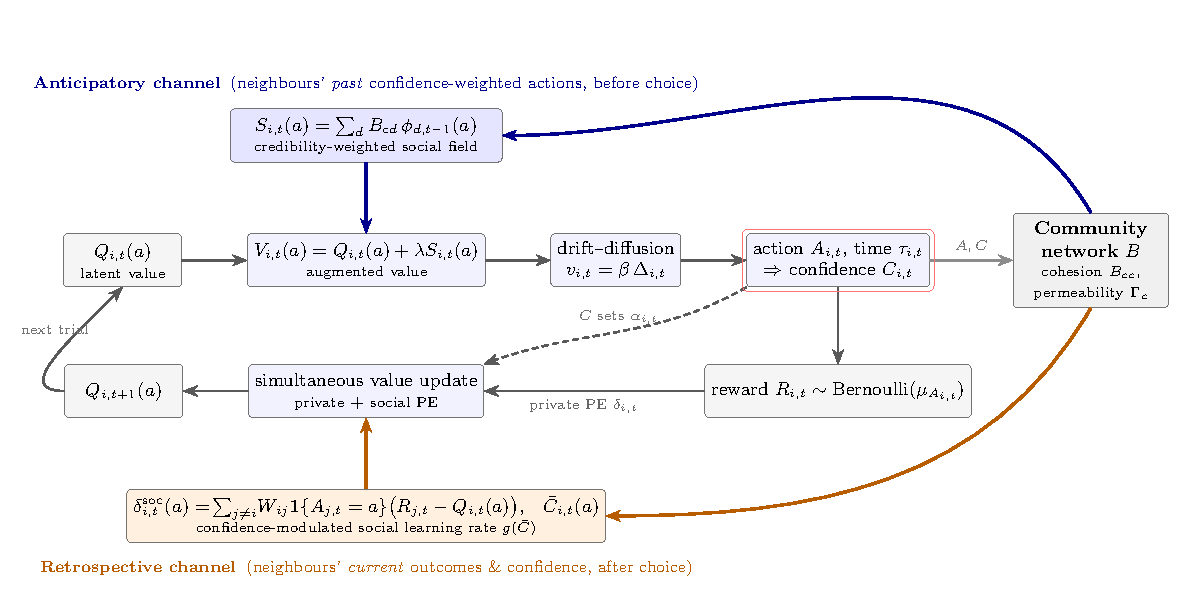
\includegraphics[width=\textwidth]{fig1_mechanism.pdf}
\caption{Mechanism. Within a trial, latent values $Q_{i,t}$ are augmented by the
anticipatory credibility field $S_{i,t}$ (top, blue) to form subjective values
$V_{i,t}$; a drift--diffusion process turns the value contrast into an action
$A_{i,t}$, a decision time $\tau_{i,t}$ and an endogenous confidence $C_{i,t}$
(red box). After the reward is observed, values are revised by a simultaneous
update combining the private prediction error with the retrospective social
prediction error (bottom, orange), whose strength is modulated by neighbours'
confidence. Confidence is the shared link between the two channels. The
community coupling matrix $B$ governs how credibility circulates.}
\label{fig:mechanism}
\end{figure}

\subsection{Purpose and entities}
The model's purpose is to explain when credibility-weighted social transmission
makes connectivity corrective and when it makes connectivity distortive. The
entities are \emph{agents} and \emph{communities}. Agents choose repeatedly
between two arms of a stochastic bandit, learn from reward, and influence one
another through a weighted communication network. Communities are an exogenous
partition of agents into modules.

\subsection{State variables and environment}
Time is discrete at the trial level, $t\in\mathbb N_0$. Agents are
$V=\{1,\dots,N\}$, partitioned into communities $V=\bigsqcup_{c=1}^M V_c$ with
$N_c=|V_c|$; community membership is $g(i)$. The action set is
$\Aset=\{1,2\}$. The weighted communication matrix
$W=(W_{ij})\in\R_+^{N\times N}$ is row-stochastic, $\sum_j W_{ij}=1$. For each
agent $i$, trial $t$ and arm $a$ we track the latent value $Q_{i,t}(a)$, the
anticipatory social signal $S_{i,t}(a)$, the augmented value $V_{i,t}(a)$, the
value contrast $\Delta_{i,t}$, the drift $v_{i,t}$, the action $A_{i,t}$, the
reward $R_{i,t}\in\{0,1\}$, the decision time $\tau_{i,t}$ and the confidence
$C_{i,t}\in(0,1)$. Arm $a$ pays Bernoulli reward with mean $\mu_a\in(0,1)$;
$a^\star\in\arg\max_a\mu_a$, $\mu^\star=\max_a\mu_a$ and $\Delta\mu=\mu_1-\mu_2$.

\subsection{Process overview and scheduling}
Each trial uses a synchronous schedule with a simultaneous post-outcome update:
(1) construct the anticipatory social signal from the previous period; (2) form
augmented values; (3) generate the drift--diffusion choice and decision time;
(4) read out confidence; (5) draw rewards; (6) compute all private and social
prediction errors from the \emph{pre-update} values; (7) apply private and
social updates simultaneously. Step~6 prevents order artefacts between private
and social revision.

\paragraph{Information structure.}
Before choosing, agents observe neighbours' previous actions and confidence
signals. After outcomes are realised, they observe neighbours' actions, realised
outcomes and confidence for the retrospective channel. Confidence is interpreted
as communicated or behaviourally inferred subjective reliability, not as
objective accuracy.

\subsection{Submodels}

\paragraph{Anticipatory social signal.}
Social information available before the current choice is
\begin{equation}
S_{i,t}(a):=\sum_{j=1}^N W_{ij}\,\1\{A_{j,t-1}=a\}\,C_{j,t-1},
\qquad S_{i,0}(a)=0,
\label{eq:Si}
\end{equation}
the confidence-weighted mass of neighbours who chose $a$ in the previous trial.
Subjective values are socially augmented,
\begin{equation}
V_{i,t}(a):=Q_{i,t}(a)+\lambda\,S_{i,t}(a),
\qquad
\Delta_{i,t}:=V_{i,t}(1)-V_{i,t}(2),
\label{eq:V}
\end{equation}
where $\lambda\ge 0$ is the anticipatory weight.

\paragraph{Process-based choice and decision time.}
Conditional on $\Delta_{i,t}$, the within-trial decision variable is a Wiener
process with drift,
\begin{equation}
\dd X_{i,t}(s)=v_{i,t}\dd s+\sigma\dd B_{i,t}(s),\quad X_{i,t}(0)=0,\quad
v_{i,t}=\beta\,\Delta_{i,t},
\label{eq:ddm}
\end{equation}
absorbed at symmetric boundaries $\pm a$; the action is $A_{i,t}=1$ if the upper
boundary is hit first and $A_{i,t}=2$ otherwise, with first-passage time
$\tau_{i,t}$. We document the implementation explicitly because confidence
depends on both drift and decision time. The choice probability is computed
\emph{exactly} from the Wiener first-passage solution,
\begin{equation}
\Prob(A_{i,t}=1)=\frac{1}{1+\exp(-2v_{i,t}a/\sigma^2)},
\label{eq:choiceprob}
\end{equation}
The choice rule \eqref{eq:choiceprob} and the mean first-passage time are
\emph{exact} (Proposition~\ref{prop:ddm}). The joint choice--time law, however,
is an \emph{approximation}: reaction times are drawn from a positive,
mean-matched inverse-Gaussian whose mean equals $\E[\tau_{i,t}]$ and whose
squared coefficient of variation is a fixed dispersion, rather than from the
exact two-boundary first-passage density. Appendix~\ref{app:tests} validates the
choice probability and the mean reaction time against a direct Euler--Maruyama
simulation of \eqref{eq:ddm}, and Appendix~\ref{app:robust} shows that regime
classification is insensitive to this approximation.

\begin{proposition}[Exact choice probability and mean decision time]
\label{prop:ddm}
For the diffusion \eqref{eq:ddm} with constant drift $v\neq0$, infinitesimal
variance $\sigma^2$ and symmetric absorbing boundaries $\pm a$ started at the
origin, the probability of absorption at $+a$ and the expected absorption time
are
\[
\Prob(A=1)=\frac{1}{1+e^{-2va/\sigma^2}},
\qquad
\E[\tau]=\frac{a}{v}\tanh\!\Big(\frac{a v}{\sigma^2}\Big),
\]
with $\E[\tau]\to a^2/\sigma^2$ as $v\to0$.
\end{proposition}

\noindent Proofs of Propositions~\ref{prop:ddm}, \ref{prop:quotient} and
\ref{prop:amplification} are collected in Appendix~\ref{app:proofs}.

\paragraph{Endogenous confidence.}
Confidence is read out from the same process and is bounded in $(0,1)$:
\begin{equation}
C_{i,t}=\Lambda\!\left(\kappa_1\frac{|v_{i,t}|}{a}
-\kappa_2\log\!\Big(1+\frac{\tau_{i,t}}{\tau_0}\Big)\right),
\qquad \Lambda(x)=\frac{1}{1+e^{-x}},
\label{eq:confidence}
\end{equation}
with $\kappa_1,\kappa_2,\tau_0>0$. Confidence rises with evidence strength and
falls with decision time. It is a subjective reliability weight and is
\emph{not} assumed to equal correctness; this separation is what allows
high-confidence error. An alternative balance-of-evidence map, in which
confidence equals the DDM probability of the chosen boundary, is used in the
ablations.

\begin{figure}[t]
\centering
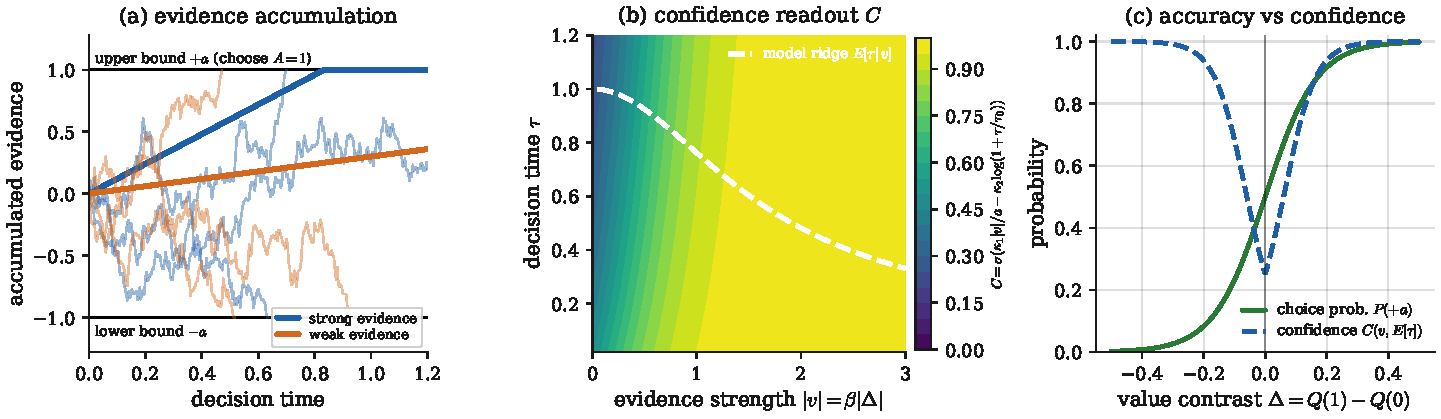
\includegraphics[width=\textwidth]{fig8_decision_confidence.pdf}
\caption{Endogenous confidence as a decision-process readout (all curves are the
exact model maps, not fits). \textbf{(a)}~Evidence accumulates to a boundary
$\pm a$ at rate $v=\beta\Delta$; strong evidence yields fast, confident choices,
weak evidence slow, uncertain ones. \textbf{(b)}~Confidence
$C=\Lambda(\kappa_1|v|/a-\kappa_2\log(1+\tau/\tau_0))$ rises with evidence
strength and falls with decision time; the dashed ridge is the process's own
mean decision time $\E[\tau\mid v]$. \textbf{(c)}~Choice accuracy $P(+a)$ is
monotone in the value contrast, but confidence is \emph{U-shaped} in $\Delta$ ---
it tracks evidence \emph{magnitude}, not correctness --- so a strongly held wrong
belief ($\Delta<0$, large) is transmitted with high credibility. This decoupling
of confidence from accuracy is the neuroeconomic root of high-confidence error.}
\label{fig:decisionconf}
\end{figure}

\paragraph{Private value revision.}
The private prediction error is $\delta_{i,t}=R_{i,t}-Q_{i,t}(A_{i,t})$, with a
confidence-modulated learning rate
\begin{equation}
\alpha_{i,t}=
\begin{cases}
\alpha^{\min}+(\alpha^{\max}-\alpha^{\min})\,C_{i,t}, & \delta_{i,t}<0,\\[2pt]
\alpha^{\max}-(\alpha^{\max}-\alpha^{\min})\,C_{i,t}, & \delta_{i,t}\ge 0,
\end{cases}
\label{eq:privatelr}
\end{equation}
so confident mistakes induce larger corrections and confident successes induce
smaller revisions, $0<\alpha^{\min}\le\alpha^{\max}<1$.

\begin{figure}[t]
\centering
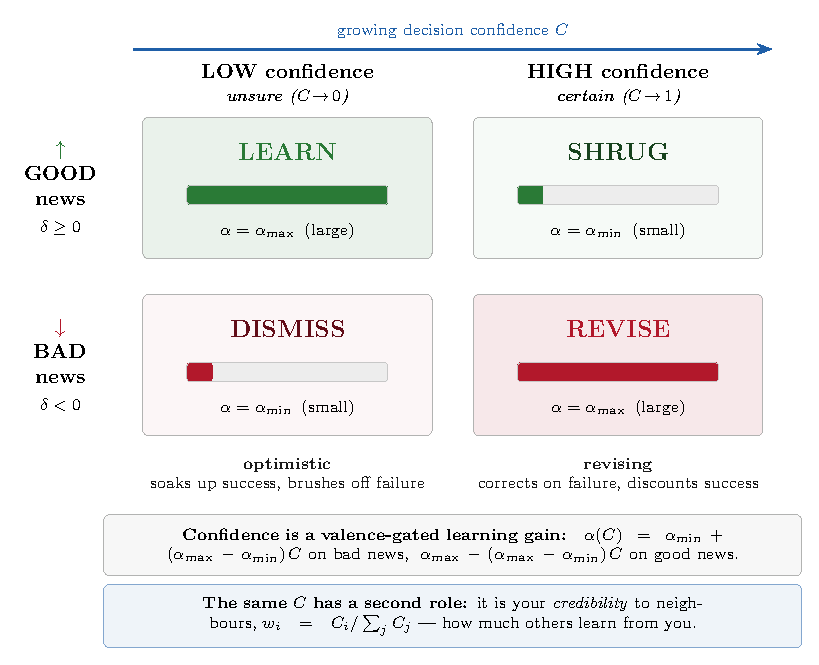
\includegraphics[width=0.82\textwidth]{fig_plasticity.pdf}
\caption{Confidence is a valence-gated learning gain. Reading the $2\times2$
matrix: the confidence-modulated learning rate \eqref{eq:privatelr} is largest
($\alpha_{\max}$) for \emph{good} news under \emph{low} confidence and for
\emph{bad} news under \emph{high} confidence, and smallest ($\alpha_{\min}$) on
the other diagonal. A low-confidence agent is therefore optimistic (soaks up
success, brushes off failure); a high-confidence agent is revising (corrects on
failure, discounts success) --- a confidence-gated analogue of asymmetric
reward-prediction-error learning. The same confidence $C$ plays a second role in
social transmission: it is the sender's credibility weight
$w_i=C_i/\sum_j C_j$, so confidence is simultaneously an intra-agent gain and an
inter-agent edge weight. The exact curves are plotted in
Appendix~\ref{app:plasticity} (Figure~\ref{fig:plasticityquant}).}
\label{fig:plasticity}
\end{figure}

\paragraph{Retrospective social learning.}
The retrospective channel uses neighbours' realised outcomes. For each arm,
\begin{equation}
\delta^{\mathrm{soc}}_{i,t}(a):=\sum_{j\neq i}W_{ij}\,\1\{A_{j,t}=a\}\bigl(R_{j,t}-Q_{i,t}(a)\bigr),
\quad
\bar C_{i,t}(a):=\frac{\sum_{j\neq i}W_{ij}\,\1\{A_{j,t}=a\}\,C_{j,t}}
{\sum_{j\neq i}W_{ij}\,\1\{A_{j,t}=a\}+\varepsilon}.
\label{eq:socpe}
\end{equation}
We adopt the convention that \emph{confidence modulates the social learning
rate} (rather than re-weighting the social prediction error itself): the social
learning rate is $g(\bar C_{i,t}(a))=\gamma\,\bar C_{i,t}(a)^{\omega}$ with
$\gamma>0,\omega>0$, $g(0)=0$. The simultaneous law of motion, with all
prediction errors formed from $Q_{i,t}$, is
\begin{equation}
Q_{i,t+1}(a)=\Pi_{[0,1]}\!\Big(
Q_{i,t}(a)+\1\{A_{i,t}=a\}\,\alpha_{i,t}\,\delta_{i,t}
+\eta\,g\!\big(\bar C_{i,t}(a)\big)\,\delta^{\mathrm{soc}}_{i,t}(a)\Big),
\label{eq:update}
\end{equation}
where $\eta\ge0$ is the retrospective weight and $\Pi_{[0,1]}$ projects onto the
reward support, keeping values interpretable as Bernoulli-mean estimates.

\paragraph{Self-weighting convention.}
We exclude an agent's own current outcome from the retrospective channel
(the sum in \eqref{eq:socpe} is over $j\neq i$), since that outcome is already
captured by the private prediction error. We \emph{include} the agent's own
previous confidence-weighted action in the anticipatory signal \eqref{eq:Si}
(so $W_{ii}\ge0$), interpreting it as choice inertia. This convention makes the
quotient field of Section~\ref{sec:quotient} exact; the verification suite tests
both inclusions (Appendix~\ref{app:tests}).

\section{Two communities and the quotient field}
\label{sec:quotient}

We first study the smallest non-trivial modular society and then generalise. For
agent $i\in V_c$ and community $d$, the block exposure is
$b_{i\to d}:=\sum_{j\in V_d}W_{ij}$, with $\sum_d b_{i\to d}=1$.

\begin{assumption}[Balanced block weights]
\label{ass:balanced}
There is a row-stochastic matrix $B=(B_{cd})_{c,d=1}^M$ with $W_{ij}=B_{cd}/N_d$
for all $i\in V_c$, $j\in V_d$.
\end{assumption}

The central mesoscopic object is the confidence-weighted action mass
\begin{equation}
\phi_{c,t}(a):=\frac1{N_c}\sum_{i\in V_c}\1\{A_{i,t}=a\}\,C_{i,t},
\label{eq:phi}
\end{equation}
which combines the fraction choosing $a$ with the average confidence carried by
those choices; we also record the action frequency
$m_{c,t}(a)=\frac1{N_c}\sum_{i\in V_c}\1\{A_{i,t}=a\}$ and the mean value
$\bar Q_{c,t}(a)$.

\begin{proposition}[Exact quotient social field]
\label{prop:quotient}
Under Assumption~\ref{ass:balanced}, for every $i\in V_c$, arm $a$ and $t\ge1$,
\begin{equation}
S_{i,t}(a)=\sum_{d=1}^M B_{cd}\,\phi_{d,t-1}(a).
\label{eq:quotientfield}
\end{equation}
In particular the anticipatory social field is identical for all agents in a
community and is a function only of the community-level masses
$\phi_{d,t-1}$.
\end{proposition}

% Proof of Proposition~\ref{prop:quotient} in Appendix~\ref{app:proofs}.

Equation~\eqref{eq:quotientfield} is the precise sense in which the community
network is a quotient of the microscopic network for the anticipatory channel.
The matrix $B$ is the community coupling matrix: its diagonal $B_{cc}$ is
\emph{cohesion}, $\Gamma_c:=1-B_{cc}=\sum_{d\neq c}B_{cd}$ is cross-community
\emph{permeability}, and $\kappa(B):=1-|\lambda_2(B)|$ is the mesoscopic mixing
rate. Computationally, \eqref{eq:quotientfield} also makes the agent-level
simulation cheap: under balanced weights both social channels reduce to
community aggregates with an $O(1/N_c)$ self-correction, so the exact dynamics
run in $O(N)$ rather than $O(N^2)$ per trial.

Defining the community contrasts
$\bar\Delta^Q_{c,t}=\bar Q_{c,t}(1)-\bar Q_{c,t}(2)$ and
$\bar\Delta^S_{c,t}=\sum_d B_{cd}(\phi_{d,t-1}(1)-\phi_{d,t-1}(2))$, the total
mesoscopic contrast $\bar\Delta_{c,t}=\bar\Delta^Q_{c,t}+\lambda\bar\Delta^S_{c,t}$
exposes the model's central tension: the private component is disciplined by
realised reward differences, while the social component amplifies whatever
confidence-weighted mass is already present.

\begin{remark}[Exact field, approximate value dynamics]
\label{rem:exact}
The field \eqref{eq:quotientfield} is exact under
Assumption~\ref{ass:balanced}. The value dynamics, however, remain stochastic
at the agent level because rewards and diffusion noise are individual. A
community-level (representative-agent) description is therefore exact for the
anticipatory field but only approximate for the full value process. We quantify
this approximation in Section~\ref{sec:results-quotient}.
\end{remark}

The quotient also yields an analytical handle on the model's central
non-monotonicity. Linearising the deterministic community recursion around the
symmetric indifference state isolates the anticipatory feedback loop.

\begin{proposition}[Local amplification threshold for the anticipatory loop]
\label{prop:amplification}
Linearise the deterministic community recursion about the symmetric indifference
state ($\bar\Delta^Q_{c,t}=0$, equal masses, equal arms). Let
$\kappa=\beta a/\sigma^2$ be the choice sensitivity, $C_0$ the confidence at the
indifference point, and $\bar b$ the effective within-community coupling. Then
the confidence-weighted mass gap $\psi_{c,t}=\phi_{c,t}(1)-\phi_{c,t}(2)$ obeys,
to first order,
\[
\psi_{c,t}=C_0\kappa\,\bar\Delta_{c,t},\qquad
\bar\Delta_{c,t}=\bar\Delta^Q_{c,t}+\lambda\,\bar b\,\psi_{c,t-1},
\]
so the anticipatory loop has one-step multiplier
$\rho(\lambda)=C_0\,\kappa\,\bar b\,\lambda$. The loop is contractive iff
$\lambda<\lambda^\star:=\sigma^2/(\beta a\,C_0\,\bar b)$. For
$\lambda<\lambda^\star$ the social field self-limits and tracks the
reward-disciplined value gap (connectivity corrective); for
$\lambda>\lambda^\star$ an early mass gap is amplified geometrically faster than
private learning can remove it (connectivity distortive).
\end{proposition}

% Proof of Proposition~\ref{prop:amplification} in Appendix~\ref{app:proofs}.

\noindent For the default parameters ($\beta=6$, $\sigma=a=1$, indifference
confidence $C_0\approx0.25$, $\bar b\approx1$) this gives
$\lambda^\star\approx0.67$, close to the corrective-to-distortive transition near
$\lambda\approx0.5$--$0.6$ in the simulated phase diagram
(Figure~\ref{fig:phase}). Combined with slow unaided learning as
$\lambda\to0$, this makes collective accuracy non-monotone in $\lambda$ and gives
the phase diagram an analytical anchor. The threshold is \emph{local}: it
predicts when small confidence-weighted mass gaps become self-amplifying around
the symmetric indifference state. It does not classify terminal regimes by
itself; the global regime map is obtained by simulation (Section~\ref{sec:results-phase}),
and an endogenous test of the threshold's predictive content --- without any
imposed early lead --- is given in Appendix~\ref{app:earlylead}.

\begin{remark}[Relation to quantal response and learning equilibria]
\label{rem:qre}
The logistic choice \eqref{eq:choiceprob} is a quantal best response to the value
contrast, so a consensus rest point of the community recursion --- action
frequencies that reproduce themselves under the choice map --- is a
quantal-response fixed point \citep{McKelveyPalfrey1995}. The corrective and
distortive regimes are stable rest points and $\lambda^\star$ marks a
bifurcation of the anticipatory map; wrong consensus is a self-confirming
non-optimal rest point, the process analogue of failures of naive learning to
aggregate information \citep{GolubJackson2010}. Agents here are non-strategic:
they do not reason about others' reasoning, so higher-order (level-$k$ /
cognitive-hierarchy) beliefs play no role. That strategic layer --- beliefs about
a representative agent, and their equilibria --- is developed in the companion
paper on legitimacy gating.
\end{remark}

\section{Simulation design}
\label{sec:design}

\paragraph{Observables and regimes.}
We measure group regret
$\mathcal R_T=\sum_{i,t\le T}(\mu^\star-\mu_{A_{i,t}})$, time to consensus, the
polarisation index $\Pi_t=|m_{1,t}(1)-m_{2,t}(1)|$, correction lag after an
early wrong lead, and, for the quotient study, the micro--meso discrepancy.
Terminal outcomes are classified into four operational regimes using a $0.9$
mass threshold: \emph{efficient consensus} (every community places
$\ge0.9$ on $a^\star$), \emph{wrong consensus} (every community places $\ge0.9$
on the suboptimal arm), \emph{polarisation} (communities lock on different
arms), and \emph{unresolved} otherwise.

\paragraph{Monte Carlo and ablations.}
Each configuration is replicated over independent reward and diffusion draws;
reported regime probabilities are frequencies over replications. The design
varies the reward gap, the anticipatory weight $\lambda$, the retrospective
weight $\eta$, cohesion and permeability. Five decisive ablations isolate the
mechanism: $\lambda=0$ (no anticipatory channel), $\eta=0$ (no retrospective
channel), constant learning rates, no confidence weighting of transmission, and
the alternative balance-of-evidence confidence map.

\subsection{Identification strategy and uncertainty}
\label{sec:identification}
Because the model is a fully specified stochastic data-generating process, the
effect of each mechanism component is a well-defined causal quantity, and we
estimate it as such rather than reading it off level differences.

\paragraph{Estimands.} We target three objects: (i) regime probabilities, the
population frequencies of each terminal regime at a configuration; (ii) means of
group regret and correction lag; and (iii) \emph{counterfactual component
effects}. Writing $\mathrm{do}(c{=}0)$ for the intervention that disables
component $c$ (the anticipatory channel, the retrospective channel, the
credibility weighting, the learning-rate modulation, or the decision-time
confidence map), the effect of $c$ on an outcome $Y$ at operating point $\theta$
is
\[
\tau_c(\theta)=\E\big[Y\mid \theta\big]-\E\big[Y\mid \theta,\ \mathrm{do}(c{=}0)\big],
\]
the difference between the factual model and the otherwise-identical model with
$c$ switched off. This is a structural, model-internal counterfactual: the
intervention changes exactly one switch and nothing else.

\paragraph{Identification by common random numbers.} We estimate $\tau_c$ by
simulating the full model and the ablation under \emph{common random numbers}.
Each replication pre-generates the same exogenous random environment --- a common
uniform reward draw and a common decision-noise draw for every agent and trial,
indexed by the same seed --- and each structural variant then realises the reward
of its chosen arm by thresholding that shared uniform at the arm's mean. The
exogenous environment is thus held fixed across variants while the endogenous
action histories are free to differ. The replication-paired difference
$D_r=Y_r(\text{full})-Y_r(\mathrm{do}(c{=}0))$ then identifies $\tau_c$ with the
exogenous environment held fixed --- a within-replication, ceteris-paribus
contrast that is the simulation analogue of a within-subject randomised
intervention. There is
no confounding because the only thing that differs between the paired runs is the
structural switch; coupling also reduces the variance of $\widehat\tau_c$
relative to independent runs. The population estimand is the one the finite-$N$
ensemble approaches as the dynamics concentrate on their mean-field limit
(Proposition~\ref{prop:amplification}; cf.\ stochastic-approximation theory
\citep{Borkar2008}).

\paragraph{Uncertainty reporting.} Regime probabilities are empirical
frequencies over independent Monte Carlo replications; we report Wilson $95\%$
intervals for binary regime probabilities and Monte Carlo standard errors with
nonparametric percentile-bootstrap $95\%$ intervals (resampling replications) for
regret and correction lag. Counterfactual contrasts $\widehat\tau_c$ carry
paired-bootstrap $95\%$ intervals (resampling replication indices jointly). Every
reported probability and mean is accompanied by its replication count $R$.

\paragraph{Verification.}
Before any result is produced, the implementation passes a ten-point test
contract (row-stochasticity of $W$ and $B$; bounded confidence; bounded values;
the simultaneous-update identity; seed reproducibility; the no-social baseline;
isolated communities $B=I$; full mixing; exactness of the quotient field; and
the self-weighting convention), together with the drift--diffusion validation
and an exact agreement check between the fast block engine and a dense-$W$
reference engine. Appendix~\ref{app:tests} lists the tests.

\paragraph{Reproducibility and scale.}
All randomness is seeded. Results below are reported at a \emph{standard}
compute scale ($N=400$ agents per two-community society, $120$--$300$
replications per configuration, $13\times13$ phase grids); the replication
package also ships a \emph{publication} scale ($N=1000$, up to $1000$
replications, $21\times21$ grids) with identical mechanism parameters. The
default parameters are listed in Appendix~\ref{app:params}.

\section{Results}
\label{sec:results}

\subsection{The mechanism produces four interpretable regimes}
\label{sec:results-baseline}
Figure~\ref{fig:baseline} shows representative two-community trajectories of the
mass placed on the optimal arm. With a clear reward gap and moderate
transmission, both communities converge on the optimal arm (efficient
consensus, $\Prob=1.00$, mean regret $450$). With a narrow gap, a strong
anticipatory weight and an early confident lead on the suboptimal arm, the same
machinery locks both communities onto the wrong arm (wrong consensus,
$\Prob=1.00$, regret $\mathbf{11{,}988}$). With near-isolated communities and
opposed early leads, the communities diverge and stay apart (polarisation,
$\Prob=1.00$, regret $5{,}998$). Each regime occurs with probability $1.00$ over
$R=300$ replications (Wilson $95\%$ lower bound $\ge0.987$;
Table~\ref{tab:baseline}). The ordering of regret across regimes ---
efficient $<$ polarisation $<$ wrong --- already shows that the costliest
outcome is not disagreement but confident, shared error.

\begin{figure}[t]
\centering
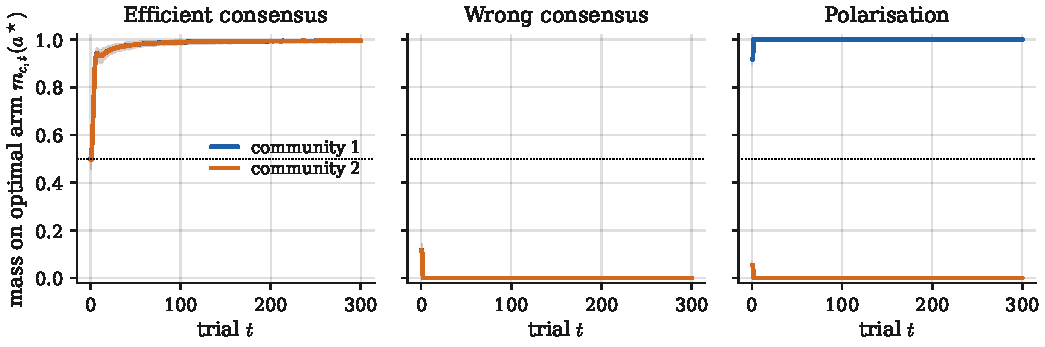
\includegraphics[width=\textwidth]{fig2_baseline.pdf}
\caption{Baseline regimes. Mass on the optimal arm $m_{c,t}(a^\star)$ in each
community (mean and $10$--$90$ percentile band over $R=300$ Monte Carlo
replications; $N=400$ agents, horizon $T=300$). The same mechanism produces
efficient consensus, wrong consensus and polarisation under the scenario
parameters of Table~\ref{tab:scenarios}.}
\label{fig:baseline}
\end{figure}

\subsection{Connectivity is non-monotone: the phase diagram}
\label{sec:results-phase}
The central result is the connectivity phase diagram
(Figure~\ref{fig:phase}), which sweeps the anticipatory weight $\lambda$ against
cross-community permeability $\Gamma$ in an asymmetric society where one
community carries an early wrong lead. Three findings stand out. First, the
effect of transmission strength is \emph{non-monotone}. At $\lambda\approx0$
lone learners fail to reach consensus within the horizon (unresolved); at
moderate $\lambda\in[0.27,0.53]$ transmission is \emph{corrective} and produces
efficient consensus across the whole permeability range; at large $\lambda$
transmission becomes \emph{distortive}. Second, the form of the distortion is
governed by permeability. At high permeability the confident wrong community
contaminates the correct one, yielding society-wide wrong consensus; at low
permeability the communities insulate one another and the society polarises.
Third, the distortive region dominates the high-$\lambda$ plane: across the grid,
wrong consensus is the modal outcome in $51\%$ of the $(\lambda,\Gamma)$ cells,
efficient consensus in $24\%$, polarisation in $9\%$ and unresolved in $15\%$.
Connectivity is thus conditionally, not uniformly, beneficial.

\begin{figure}[t]
\centering
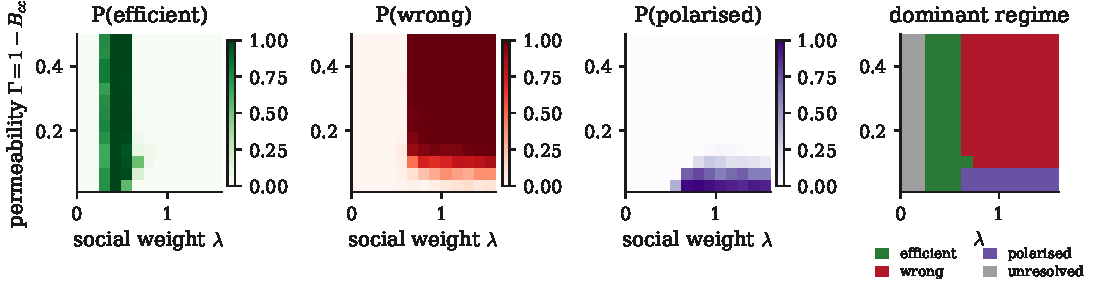
\includegraphics[width=\textwidth]{fig3_phase.pdf}
\caption{Connectivity phase diagram. Probability of efficient consensus, wrong
consensus and polarisation, and the dominant regime, over the anticipatory
weight $\lambda$ and cross-community permeability $\Gamma=1-B_{cc}$. A corrective
band at moderate $\lambda$ separates an unresolved region ($\lambda\to0$) from a
distortive region (large $\lambda$); within the distortive region, low
permeability yields polarisation and high permeability yields wrong consensus.
Grid $13\times13$, $120$ replications per cell, regime threshold $0.9$, horizon
$T=240$; the first three panels show regime probabilities and the fourth the
dominant (modal) regime. The Wilson half-width at $120$ replications is at most
$0.09$.}
\label{fig:phase}
\end{figure}

\subsection{A dynamical-systems view: bifurcation and phase portrait}
\label{sec:dynamics}
The stochastic model admits an exact large-population ($N\to\infty$) reduction on
balanced blocks (\texttt{credibility/meanfield.py}): within a community all agents
share the same expected value table, choices are replaced by the exact DDM
probability $\Lambda(2\beta a\Delta/\sigma^2)$, decision times by the mean
first-passage time, and rewards by their means. Freezing values at the
indifference point isolates the object of Proposition~\ref{prop:amplification}:
the anticipatory feedback on the population lead $z_c=m_c(0)-\tfrac12$. The
symmetric mode has gain $\beta a\lambda\bar b\,C_0/\sigma^2$, which crosses one at
$\lambda^\star=\sigma^2/(\beta a C_0\bar b)$; because the block coupling is
row-stochastic, $\bar b=1$ for a common lead and permeability enters only the
anti-symmetric modes.

Figure~\ref{fig:bifurcation} shows the resulting bifurcation: below
$\lambda^\star$ the neutral state $z=0$ is stable and small early leads decay
(links are corrective); above $\lambda^\star$ it loses stability and a symmetric
pair of amplified fixed points appears --- $+z^\star$ a confidently correct
consensus, $-z^\star$ a confidently wrong one --- so the \emph{same} links that
corrected now lock in whichever early lead exists. The flow field
(Figure~\ref{fig:flowfield}) shows the same transition through its fixed points:
a single attracting neutral state below $\lambda^\star$, and above it a repelling
neutral state with four corner attractors (corrective, distortive, two
polarised). The basin portrait (Figure~\ref{fig:vectorfield}) then shows this
reorganisation of the flow across a sweep of $\lambda$.
Below $\lambda^\star$ the entire early-lead plane drains to the neutral state:
connectivity corrects any initial asymmetry. Above $\lambda^\star$ the neutral
state becomes a saddle and the plane partitions into four basins of attraction
--- corrective, distortive and two polarised corners --- so the \emph{position}
of the early lead, not its mere presence, now decides the collective outcome.
As $\lambda$ grows the corrective and distortive basins enlarge at the expense of
the polarised ones. This is the mechanism of Figure~\ref{fig:phase} in
miniature: the permeability $\Gamma$ tilts the basin boundaries (a weakly coupled
community resists an infected neighbour, favouring polarisation), while the
finite-$N$ fluctuations of the agent model scatter the early lead across the
plane, so the basin areas become the regime frequencies measured there.

\begin{figure}[t]
\centering
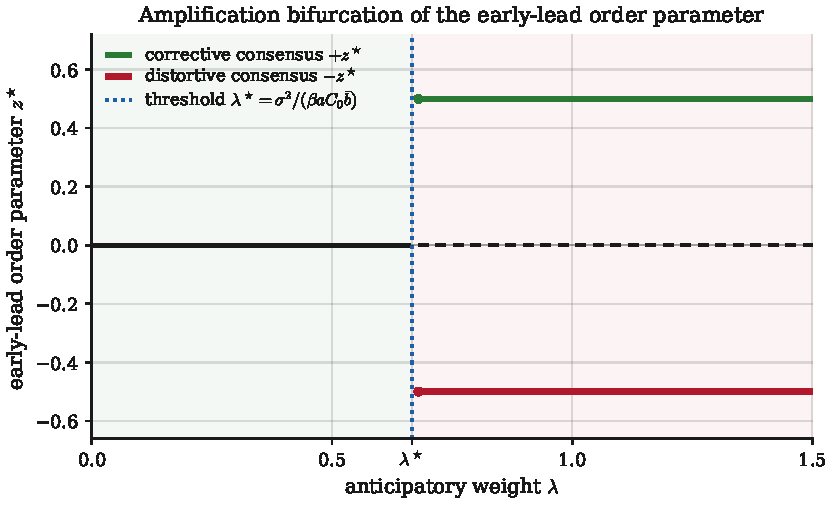
\includegraphics[width=0.72\textwidth]{fig12_bifurcation.pdf}
\caption{Amplification bifurcation of the mean-field reduction. The early-lead
order parameter $z^\star$ is zero (stable neutral state) below $\lambda^\star$
and splits into a correct ($+z^\star$) and a wrong ($-z^\star$) amplified branch
above it. The transition is mildly subcritical (a bistable window precedes
$\lambda^\star$), so a sufficiently large early lead can lock in just below
threshold. Small reward gap $|\Delta\mu|=0.06$, $B_{cc}=0.85$.}
\label{fig:bifurcation}
\end{figure}

\begin{figure}[t]
\centering
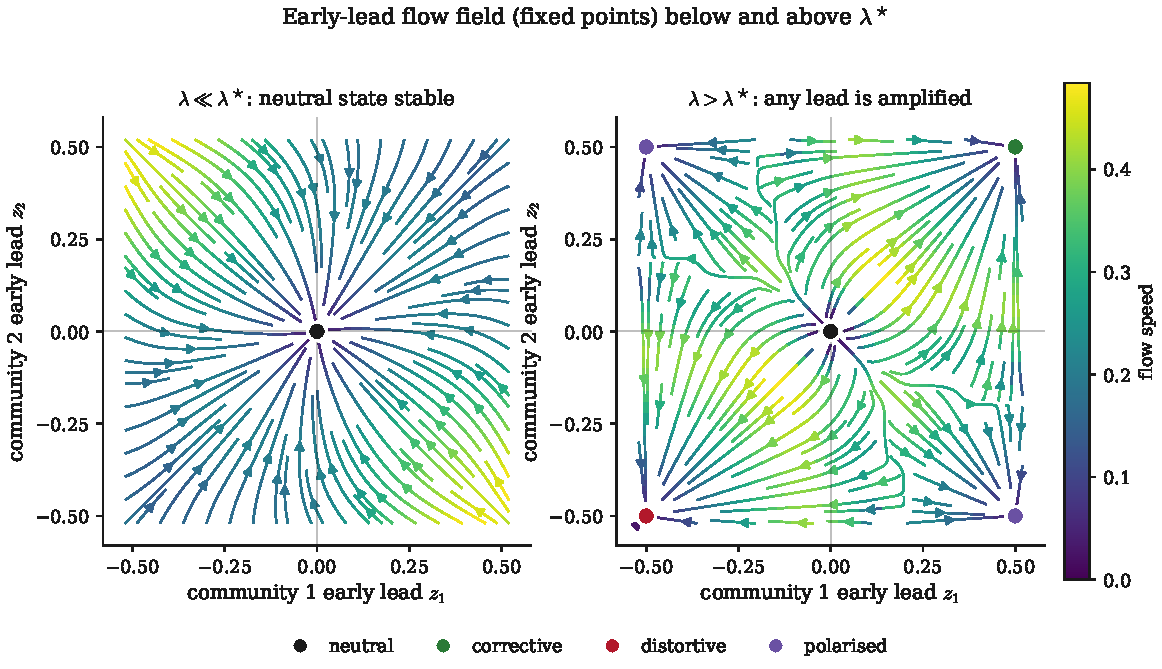
\includegraphics[width=0.86\textwidth]{fig13_flowfield.pdf}
\caption{Early-lead flow field of the mean-field reduction, streamlines coloured
by speed with the fixed points marked. \textbf{(left)}~$\lambda\ll\lambda^\star$:
the neutral state $(0,0)$ is the sole attractor. \textbf{(right)}~$\lambda>\lambda^\star$:
the neutral state is a source and four attractors appear --- corrective $(+,+)$,
distortive $(-,-)$ and two polarised $(\pm,\mp)$ corners. Frozen-value reduction,
$|\Delta\mu|=0.06$, $B_{cc}=0.85$.}
\label{fig:flowfield}
\end{figure}

\begin{figure}[t]
\centering
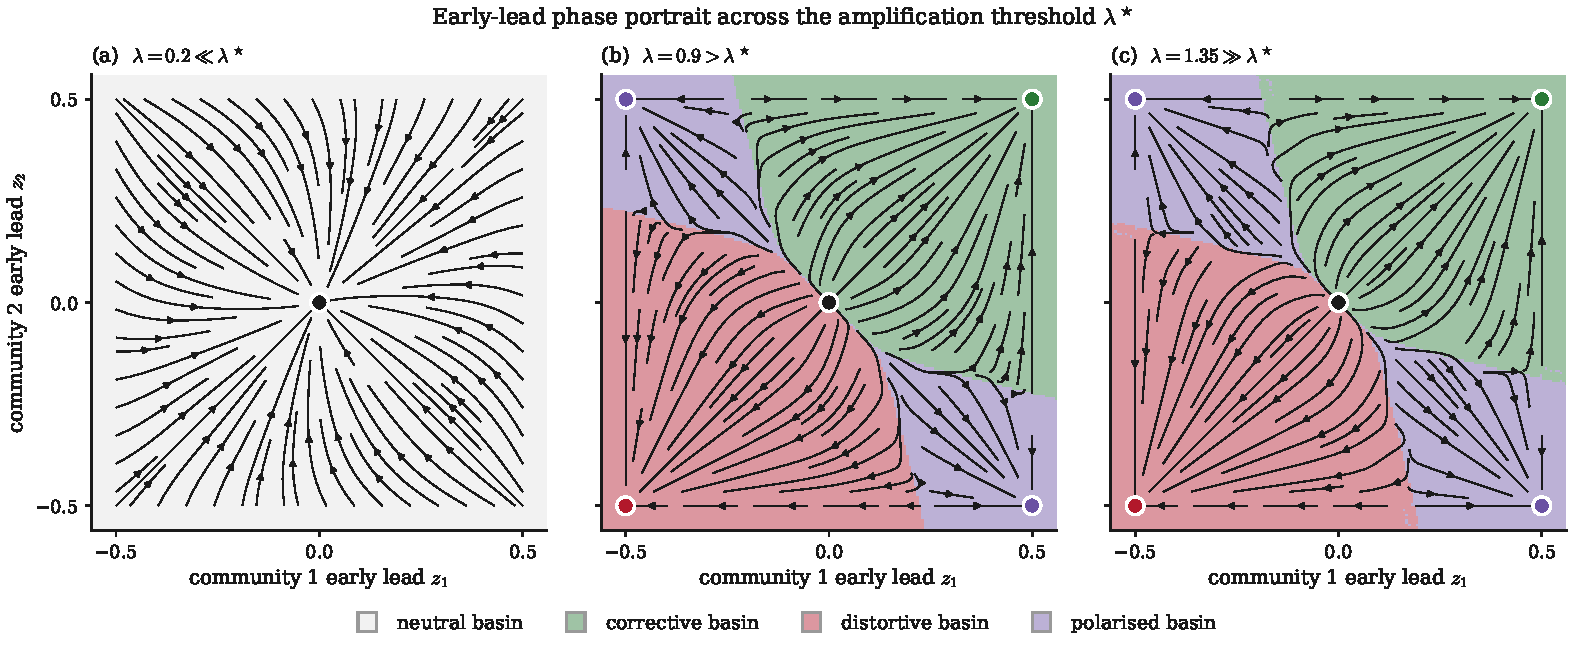
\includegraphics[width=\textwidth]{fig13_vectorfield.pdf}
\caption{Early-lead phase portrait of the mean-field reduction across the
amplification threshold. Axes are the two communities' early leads $(z_1,z_2)$;
streamlines show the flow and shading marks each point's basin of attraction
(neutral, corrective, distortive, polarised). \textbf{(a)}~$\lambda\ll\lambda^\star$:
the whole plane drains to the neutral state --- connectivity corrects any early
asymmetry. \textbf{(b)}~$\lambda>\lambda^\star$: the neutral state is a saddle and
the plane splits into four basins, so the \emph{location} of the early lead sets
the outcome. \textbf{(c)}~$\lambda\gg\lambda^\star$: the corrective and distortive
basins expand and the polarised basins shrink. Frozen-value reduction,
$|\Delta\mu|=0.06$, $B_{cc}=0.85$.}
\label{fig:vectorfield}
\end{figure}

\subsection{The wrong-consensus regime requires the full mechanism}
\label{sec:results-ablation}
We isolate each component using the counterfactual design of
Section~\ref{sec:identification}: the full model and five ablations are run under
common random numbers ($R=300$) at a contested operating point where the full
model produces wrong consensus with probability $0.83$ (Wilson $95\%$ interval
$[0.78,0.87]$). Figure~\ref{fig:ablations} and Table~\ref{tab:ablation} report
the per-variant regimes and the paired counterfactual effects
$\widehat\tau_c=\mathrm{P}(\text{wrong}\mid\text{full})-\mathrm{P}(\text{wrong}\mid\text{ablation})$.
The components fall into three classes, and every paired interval excludes zero.
\emph{Necessary} components, whose removal eliminates the distortion: disabling
the anticipatory channel ($\lambda=0$), the retrospective channel ($\eta=0$), or
the decision-time dependence of confidence (the balance-of-evidence map) each
drives wrong consensus to $0.00$, a paired effect $\widehat\tau_c=+0.83$
($[0.79,0.87]$) with group regret an order of magnitude lower.
\emph{Contributory but not necessary}: removing the credibility weighting of
transmission \emph{weakens but does not eliminate} the distortion (wrong
consensus $0.83\!\to\!0.73$, $\widehat\tau=+0.10$, $[0.04,0.16]$).
\emph{Buffering}: holding learning rates constant \emph{intensifies} the
distortion (wrong consensus $0.83\!\to\!0.99$, $\widehat\tau=-0.16$,
$[-0.21,-0.12]$), because the confidence-modulated rate of \eqref{eq:privatelr},
which enlarges corrections after confident mistakes, is the model's main private
brake on error. The wrong-consensus regime is therefore not a generic feature of
social learning: it is specific to the full confidence-weighted, dual-channel
mechanism, and credibility weighting modulates rather than creates it.

\begin{figure}[t]
\centering
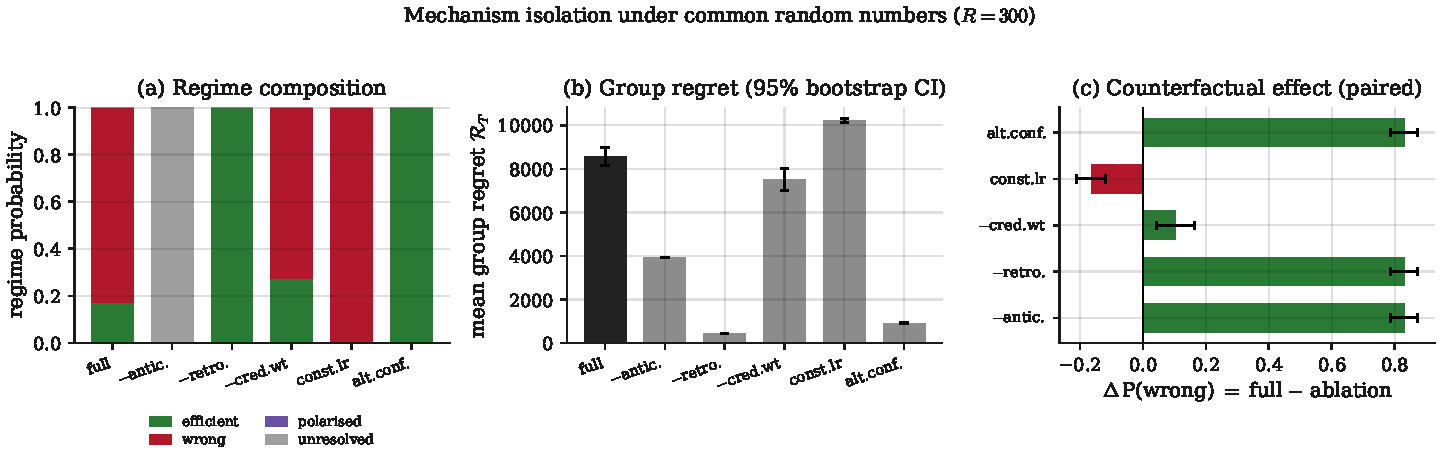
\includegraphics[width=\textwidth]{fig4_ablations.pdf}
\caption{Mechanism isolation under common random numbers ($R=300$). (a) Regime
composition for the full model and five ablations at the contested operating
point (Table~\ref{tab:scenarios}); (b) mean group regret with $95\%$ bootstrap
intervals; (c) paired counterfactual effect on wrong consensus,
$\Delta\mathrm{P(wrong)}=\text{full}-\text{ablation}$, with paired-bootstrap
$95\%$ intervals (green: the component is necessary for the distortion; red: the
component buffers against it). Removing the anticipatory channel, the
retrospective channel, or the decision-time confidence map eliminates wrong
consensus; removing credibility weighting only weakens it; constant learning
rates intensify it.}
\label{fig:ablations}
\end{figure}

\subsection{Confidence attaches to error}
\label{sec:results-confidence}
Why can transmission distort? Because confidence is endogenous and can attach to
wrong choices early in learning, exactly as the mechanism requires.
Figure~\ref{fig:confidence} shows the distribution of confidence conditional on
whether the chosen arm was optimal, split by phase. Early in learning, wrong choices carry substantial confidence
(mean $0.73$, with appreciable mass above $0.9$), only modestly below the
confidence of correct choices (mean $0.98$). These early confident errors are
precisely the signals that the anticipatory channel amplifies before enough
corrective evidence has accumulated. The mechanism requires no global
irrationality --- only that early stochastic success can generate confidence,
and that confidence is socially read as credibility.

\begin{figure}[t]
\centering
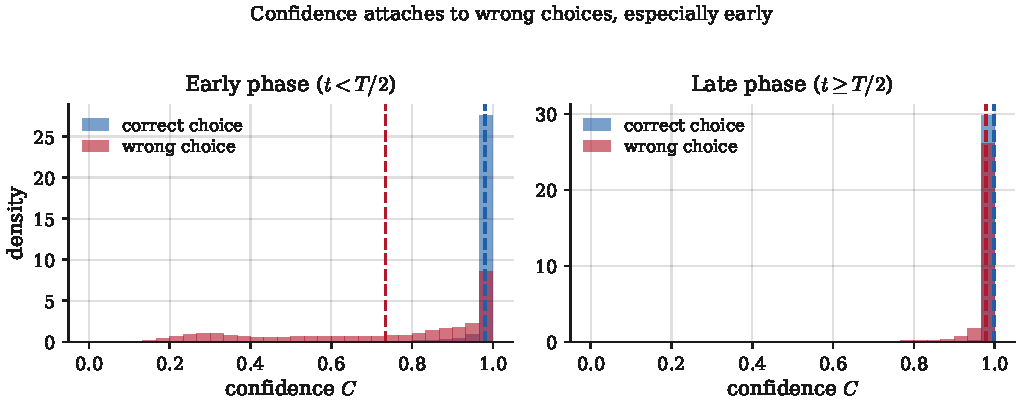
\includegraphics[width=\textwidth]{fig5_confidence.pdf}
\caption{Endogenous confidence and early confident error. Distribution of
confidence $C$ for correct and wrong choices, early ($t<T/2$) and late
($t\ge T/2$), in a neutral contested scenario; densities are normalised to unit
area and dashed lines mark group means. Early decisions number $\approx1.8\times10^6$
(correct) and $\approx6\times10^4$ (wrong). Early wrong choices carry a wide
range of confidence, including high values (mean $0.73$ versus $0.98$ for correct
choices): confidence attaches to error, which is what lets credibility-weighted
transmission amplify it. The right panel shows that confidence concentrates near
one late in learning as communities reach consensus.}
\label{fig:confidence}
\end{figure}

\subsection{The community quotient is faithful in the bulk and breaks at boundaries}
\label{sec:results-quotient}
Finally we validate the community-level (quotient) description against the full
agent model (Figure~\ref{fig:quotient}). In two- and four-community examples the
deterministic meso recursion tracks the micro ensemble mean closely, including a
modular four-community society in which both descriptions reach the optimal arm
(terminal micro mass $0.997$ per community versus meso $1.000$). Across a
$(\lambda,\Gamma)$ sweep the mean absolute discrepancy between the micro
ensemble and the meso trajectory is $0.137$, and the two descriptions agree on
the dominant regime in $79\%$ of cells. Consistent with
Remark~\ref{rem:exact}, the discrepancy is small in the interior of regimes and
concentrates along the corrective/distortive phase boundary near
$\lambda\approx0.5$, where finite-$N$ fluctuations decide the regime and the
deterministic reduction is least reliable. The quotient is thus a useful but
bounded instrument: exact for the anticipatory field, accurate for aggregate
behaviour away from transitions, and explicitly not a substitute for the
agent-level model near them.

\begin{figure}[t]
\centering
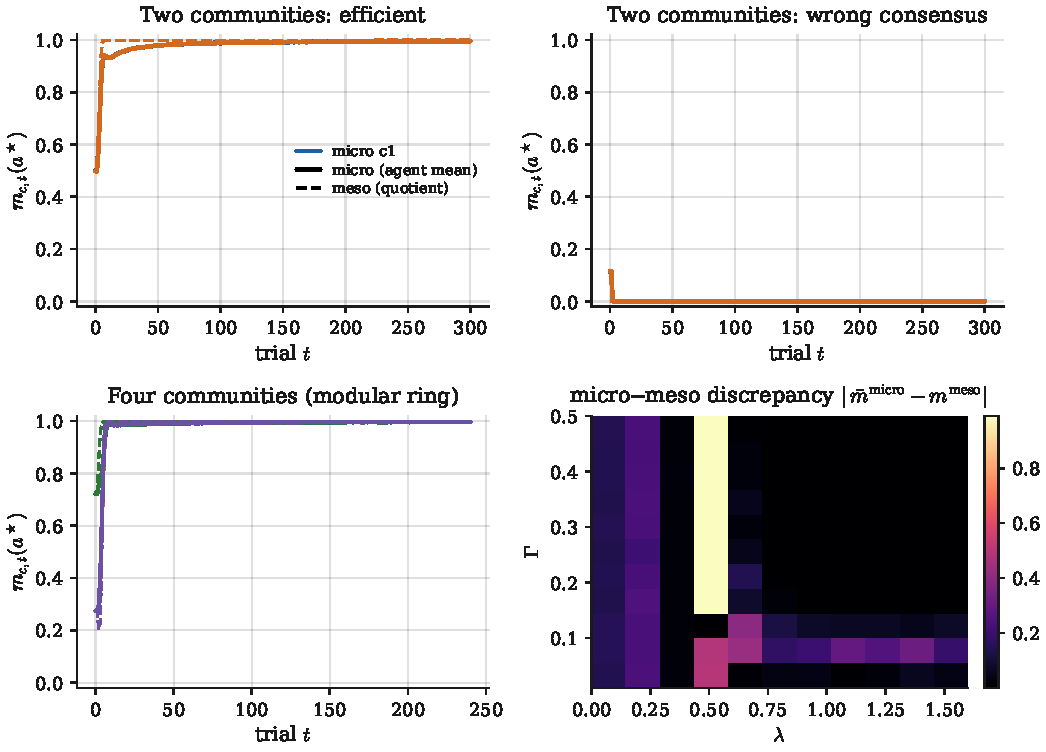
\includegraphics[width=\textwidth]{fig6_quotient.pdf}
\caption{Micro--meso validation. Agent-level ensemble mean (solid) versus the
deterministic quotient (dashed) for two-community efficient and wrong consensus
and a four-community ($M=4$) modular ring. Bottom-right: the micro--meso
discrepancy $\frac1M\sum_c|\bar m^{\mathrm{micro}}_{c,T}(a^\star)-m^{\mathrm{meso}}_{c,T}(a^\star)|$
over an $11\times11$ $(\lambda,\Gamma)$ grid ($\approx66$ replications per cell).
Mean discrepancy $0.137$ and dominant-regime agreement $79\%$; the error
concentrates along the corrective/distortive boundary near $\lambda\approx0.5$.}
\label{fig:quotient}
\end{figure}

\subsection{Robustness}
\label{sec:results-robustness}
The phase structure is robust (Appendix~\ref{app:robust},
Table~\ref{tab:robustness}, Figure~\ref{fig:robustness}). Across terminal
thresholds ($0.80/0.90/0.95$), horizons ($T$ up to $1000$), reward gaps
($|\Delta\mu|$ from $0.02$ to $0.20$), and moderate perturbations away from
balanced block weights (weighted stochastic-block and noisy row-normalised
graphs), the corrective, distortive and polarised regimes persist, and the
dominant-regime map is essentially unchanged across phase-grid resolutions and
under a deterministic reaction-time approximation. The unresolved region at
$\lambda\to0$ is genuine rather than slow convergence: it persists at $T=1000$.
The principal sensitivity is to the strength of the early lead: at the distortive
operating point even a small initial asymmetry ($\delta=0.04$) is sufficient to
produce wrong consensus, consistent with the amplification threshold of
Proposition~\ref{prop:amplification}. The largest residual uncertainty sits, as
expected, on the corrective/distortive boundary, where finite-$N$ fluctuations
and the quotient approximation are least reliable.

% Auto-generated by scripts/make_tables.py -- do not edit.
\begin{table}[t]\centering\small
\caption{Baseline regimes. Each scenario is run for $R$ Monte Carlo replications; the realised regime probability is $1.00$ in every case, reported with its Wilson 95\% lower bound. $\mathcal{R}_T$ is mean group regret with Monte Carlo standard error. Scenario parameters are in Table~\ref{tab:scenarios}.}
\label{tab:baseline}
\begin{tabular}{lcccc}\toprule
Regime & $R$ & $\lambda$ & P(regime) [Wilson 95\% LB] & $\mathcal{R}_T$ (SE) \\ \midrule
efficient & 300 & 0.40 & $1.00$ [0.987] & 450 (1) \\
wrong & 300 & 0.90 & $1.00$ [0.987] & 11,988 (0) \\
polarised & 300 & 0.90 & $1.00$ [0.987] & 5,998 (0) \\
\bottomrule\end{tabular}
\end{table}
\begin{table}[t]\centering\small
\caption{Mechanism isolation at the contested operating point (Table~\ref{tab:scenarios}), $R=300$ replications under common random numbers. P(wrong) and P(efficient) carry Wilson 95\% intervals; regret carries a 95\% bootstrap interval. The last column is the paired counterfactual effect on wrong consensus, $\Delta=$P(wrong$\mid$full)$-$P(wrong$\mid$ablation), with a paired bootstrap 95\% interval. A positive $\Delta$ whose interval excludes $0$ means the component is necessary for the distortion.}
\label{tab:ablation}
\begin{tabular}{lcccc}\toprule
Variant & P(wrong) [95\%] & P(eff.) [95\%] & $\mathcal{R}_T$ [95\%] & $\Delta$P(wrong) [95\%] \\ \midrule
full & 0.83 [0.78, 0.87] & 0.17 [0.13, 0.22] & 8,571 [8,148, 8,962] & --- \\
no anticipatory & 0.00 [0.00, 0.01] & 0.00 [0.00, 0.01] & 3,913 [3,908, 3,919] & $+0.83$ [+0.79, +0.87] \\
no retrospective & 0.00 [0.00, 0.01] & 1.00 [0.99, 1.00] & 438 [433, 442] & $+0.83$ [+0.79, +0.87] \\
no credibility wt. & 0.73 [0.67, 0.77] & 0.27 [0.23, 0.33] & 7,501 [7,002, 7,996] & $+0.10$ [+0.04, +0.16] \\
constant LR & 0.99 [0.98, 1.00] & 0.01 [0.00, 0.02] & 10,239 [10,142, 10,303] & $-0.16$ [-0.21, -0.12] \\
alt.\ confidence & 0.00 [0.00, 0.01] & 1.00 [0.99, 1.00] & 911 [882, 941] & $+0.83$ [+0.79, +0.87] \\
\bottomrule\end{tabular}
\end{table}


\section{Discussion}
\label{sec:discussion}

The simulations support four claims.

\emph{Connectivity is conditionally beneficial.} The relationship between
social transmission and collective accuracy is non-monotone
(Figure~\ref{fig:phase}). A corrective band of moderate credibility-weighted
transmission separates an unresolved regime, in which agents have too little
social information to converge, from a distortive regime, in which they have too
much. The policy-relevant reading is that interventions which simply increase
connectivity can move a society from the corrective band into the distortive
region.

\emph{Confidence is an endogenous amplifier, not a report.} Because confidence
is produced by the decision process and can attach to error
(Figure~\ref{fig:confidence}), social transmission is not neutral pooling. When
credibility tracks accuracy it accelerates correction; when it tracks early,
mistaken conviction it manufactures wrong consensus. The ablations
(Figure~\ref{fig:ablations}) show that this depends on the specific way
confidence is generated and used: the decision-time dependence of confidence and
the confidence-modulated learning rate are not decorative.

\emph{Modularity both protects and entrenches.} Low cross-community permeability
prevents a confident wrong community from contaminating its neighbour, but the
same insulation converts contagion into persistent polarisation
(Figure~\ref{fig:phase}). Modularity therefore trades one failure mode for
another rather than removing failure.

\emph{Quotient aggregation is useful but limited.} The community description is
exact for the anticipatory social field (Proposition~\ref{prop:quotient}) and
faithful for aggregate behaviour away from phase boundaries, but it is only an
approximation of the stochastic value dynamics and degrades precisely where
regime selection is decided (Figure~\ref{fig:quotient}). Mesoscopic reasoning
about this class of models should be used for bulk behaviour and checked against
the agent model near transitions.

\paragraph{Cognitive interpretation.}
The parameters carry direct cognitive readings: $\beta$ is value sensitivity
(how sharply value differences drive choice), $\sigma$ internal decision noise,
$a$ the speed--accuracy threshold, $\kappa_1,\kappa_2$ the evidence- and
time-dependence of confidence, $\alpha$ the reward learning rate, $\lambda$
susceptibility to social influence, and $\eta$ retrospective credit assignment
(Appendix~\ref{app:params}). The retrospective channel is an other-referenced
prediction error, the social counterpart of the reward prediction error
\citep{JoinerPivaTurrinChang2017}, and the confidence-modulated learning rule is
a teaching-like signal in the sense of orbitofrontal adaptive-learning accounts
\citep{SchuckCaiWilsonNiv2016,Niv2019,WangVeismannBanerjeePleger2023}. The model
tracks action values rather than latent task states; relating credibility
transmission to belief-state or cognitive-map inference
\citep{Niv2019,BehrensMullerWhittingtonMarkSchultzeDolanKurthNelson2018} is a
natural theoretical extension.

\paragraph{A normative benchmark.}
Group regret measures the summed reward shortfall relative to the omniscient
optimum (zero regret). Against a \emph{non-social} benchmark --- the same agents
with $\lambda=\eta=0$ (pure reinforcement learning) at matched environments ---
credibility-weighted social learning is doubly signed: in the corrective regime
it cuts mean regret from about $7{,}400$ (non-social) to $450$, a $16$-fold
improvement toward the ideal observer; in the distortive regime it inflates
regret from about $4{,}800$ (non-social) to $12{,}000$, roughly $2.5$ times
worse. Confidence-weighted transmission thus approaches the optimum when
credibility tracks accuracy and departs from both the optimum and the non-social
learner when it amplifies early error --- a precise statement of when the
mechanism is beneficial versus pathological.

\paragraph{Testable predictions.}
The mechanism yields experiment-ready predictions. \textbf{(i)} High-confidence
individuals should disproportionately influence collective learning, because
credibility weights transmission by confidence. \textbf{(ii)} Early overconfident
errors should produce persistent herd effects: above the local amplification
threshold an early confident wrong lead locks in
(Figure~\ref{fig:earlylead}). \textbf{(iii)} Raising decision uncertainty ---
lowering confidence by degrading evidence or shortening deliberation --- should
reduce social contagion, since the anticipatory field is confidence-weighted.
\textbf{(iv)} Manipulating confidence \emph{independently of accuracy} (removing
credibility weighting, or the balance-of-evidence confidence map) should change
network dynamics without changing individual accuracy
(Figure~\ref{fig:ablations}). \textbf{(v)} Because confidence is never observed
directly but \emph{inferred}, a receiver's weighting of a sender should track
observable proxies of latent confidence --- short reaction times, absence of
choice vacillation, and past reliability --- \emph{controlling for} the sender's
accuracy; masking those cues (hiding reaction time, adding response jitter,
resetting reputation) should attenuate transmission even when accuracy is fixed.
The confidence map itself makes this quantitative: since $C$ falls with decision
time (Eq.~\ref{eq:confidence}), following should decrease monotonically in a
sender's reaction time at matched evidence. Each maps onto a manipulable quantity
in group-decision experiments.

\paragraph{A neuroeconomic reading.}
The model's variables line up, one for one, with quantities that decision
neuroscience already measures (Figure~\ref{fig:neuromap}): a value contrast
driving an accumulator, a bounded-integration choice, a confidence readout, a
reward prediction error, a confidence-gated learning gain, and a
credibility-weighted \emph{social} prediction error of the kind reported for
other-referenced error signals \citep{JoinerPivaTurrinChang2017}. The mapping is
a functional analogy: the model commits to the computations, the substrates are
candidate correlates. Its use is to turn predictions \emph{(i)--(iv)} into a
concrete, model-based experimental design (Figure~\ref{fig:experiment}). Confidence is manipulated orthogonally to accuracy
--- by speed pressure, evidence-quality framing, or an explicit confidence
display --- populating a confident-error cell that a purely accuracy-driven
account cannot produce. The model then supplies the regressors (decision
confidence $C_{i,t}$, private PE $\delta_{i,t}$, and the credibility-weighted
social PE) for a model-based analysis of behaviour or neural signal, with the
sharp prediction that a receiver's movement scales with sender confidence
\emph{controlling for} correctness. Because the transmitted confidence is a
\emph{latent} variable, the same design supports a hierarchical latent-variable
analysis: estimate each sender's trial-by-trial confidence from reaction time,
explicit report and choice history, then test whether the receiver's social
prediction error is weighted by this \emph{inferred} confidence rather than by
observed accuracy. This turns the assumption that confidence is directly observed
into an identifiable estimand and a falsifiable test of the credibility channel.

\begin{figure}[t]
\centering
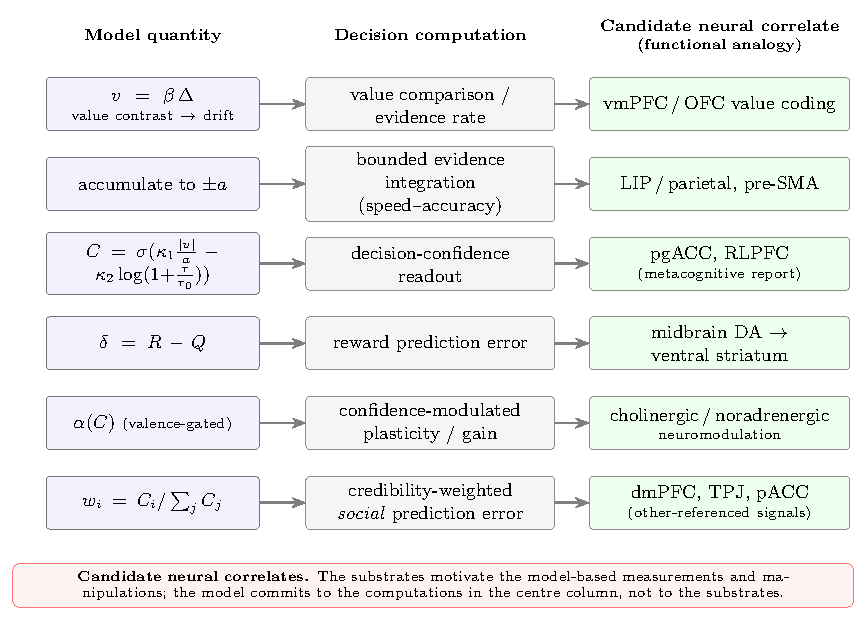
\includegraphics[width=\textwidth]{fig10_neuromap.pdf}
\caption{Computational-to-neural correspondence. Each model quantity (left)
implements a decision computation (centre) with a candidate neural correlate
(right). A functional analogy: it motivates the measurements and manipulations of
Figure~\ref{fig:experiment}; the model commits to the centre column.}
\label{fig:neuromap}
\end{figure}

\begin{figure}[t]
\centering
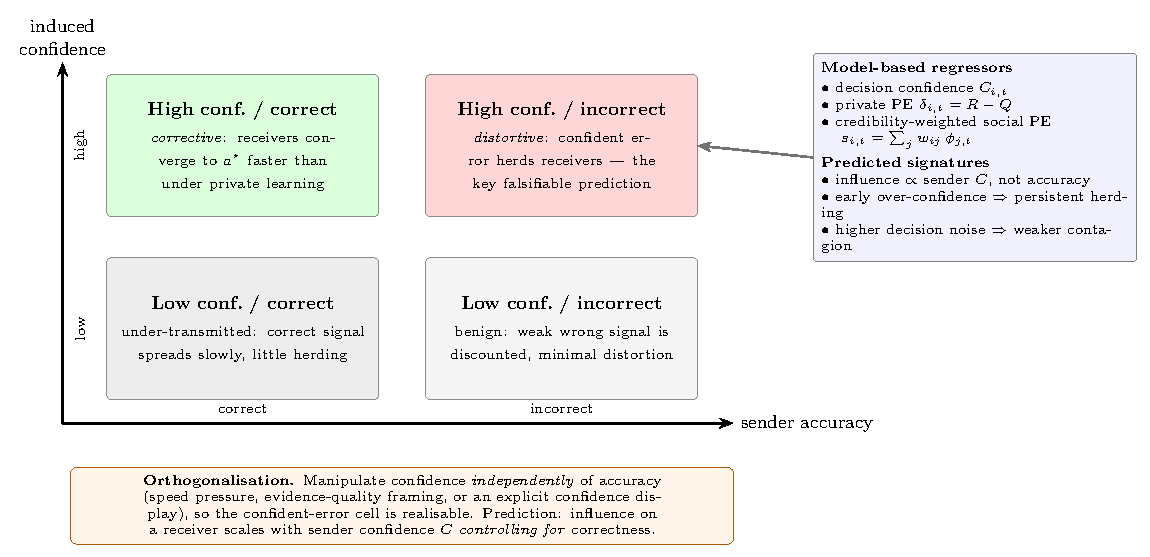
\includegraphics[width=\textwidth]{fig11_experiment.pdf}
\caption{A model-based experimental design. Inducing confidence orthogonally to
accuracy realises the confident-error cell (upper right), where the model
predicts distortive transmission. The model supplies the regressors and
falsifiable signatures (right), turning predictions \emph{(i)--(iv)} into a
testable protocol for dyadic or networked group-decision experiments.}
\label{fig:experiment}
\end{figure}

\paragraph{Limitations and scope.}
The baseline is deliberately narrow: binary actions, stationary rewards, fixed
networks, community-homogeneous parameters, and a progression from two
communities to a modular ring. Four assumptions are cognitively strong and each
suggests an extension. Neighbours' confidence enters transmission as if directly
observed, whereas confidence is usually \emph{inferred} from reaction time,
hesitation, or past reliability; we recast this as testable prediction~(v) and a
latent-variable estimand above, and a fully generative model that infers
transmitted confidence from these cues is a natural next modelling step. The anticipatory and
retrospective channels are kept independent, but exposure to a confident
neighbour before a choice plausibly changes how later feedback is weighted, so
the channels may interact. The network is fixed, whereas real influence weights
adapt as agents learn whom to trust; endogenous, reputation-driven weights would
make the model richer. And confidence here only modulates learning, whereas low
confidence also promotes exploration and high confidence exploitation, a further
behavioural role worth adding. Each extension should earn its place by the
limitation it removes and the observable that identifies its effect, added only
after the present mechanism is held fixed.

\paragraph{Boundary of the present model.}
The model deliberately stops before legitimacy. Agents may be wrong,
overconfident, or socially amplified, but they do not dispute the
reward-generating rule itself. Realised rewards remain valid evidence for value
revision. This boundary is useful because it isolates credibility transmission
as a mechanism of collective error. It also identifies the next modelling step:
if agents can discount rewards because they regard the rule as unfair, social
learning becomes a joint process of value learning and legitimacy learning.

\paragraph{From credibility to legitimacy (future work).}
A natural extension is to relax the assumption that reward feedback is always
treated as a legitimate learning signal. In the present model, prediction errors
discipline latent values directly. In many social settings, however, a confident
failure may be interpreted not as evidence that one's belief was wrong, but as
evidence that the rule assigning rewards is unfair
\citep{Rabin1993Fairness,FehrSchmidt1999,BoltonOckenfels2000}. This could be
modelled by introducing a latent legitimacy state that gates the effective
prediction error, together with a perceived fairness benchmark defined relative
to a representative modal agent. Agents would then learn not only which actions
pay, but also whether the payoff rule is acceptable. Network geometry would
modulate the diffusion of both credibility and fairness benchmarks, potentially
generating legitimacy polarisation, defensive wrong consensus, or correct but
illegitimate consensus. This extension is left for future work.

\section{Conclusion}
We have presented an implemented agent-based model of social learning in which
confidence is generated endogenously by a drift--diffusion decision process and
transmitted socially as credibility through two distinct channels. The model is
verified against an explicit test contract and studied by Monte Carlo
simulation. Its central finding is that connectivity is non-monotone and
conditional: moderate credibility-weighted transmission corrects error, while
strong transmission amplifies early overconfident mistakes into wrong consensus
or, under low permeability, into persistent polarisation. The same network links
carry correction or distortion depending on whether the circulating credibility
tracks accuracy or early error. A replication package regenerates every result.
Future work can relax the assumption that rewards remain legitimate evidence and
study when credibility-weighted communities learn not only which actions pay, but
whether the payoff rule itself is acceptable.

\section*{Code and data availability}
All code, configurations, fixed seeds and analysis scripts that reproduce every
figure and table are released as the open-source \textsc{csl} (Cognitive Social
Learning) repository under an MIT license:
\url{https://github.com/<owner>/CSL} (release tag and archive DOI to be inserted
on publication). The repository documents the verification suite, the
common-random-number ablation protocol, and one-command reproduction of the
standard and publication profiles.

\appendix

\section{Proofs}
\label{app:proofs}

\begin{proof}[Proof of Proposition~\ref{prop:ddm}]
Let $s(x)=e^{-2vx/\sigma^2}$ be the Wiener scale function; then $s(X_t)$ is a
bounded local martingale up to the exit time $\tau$ of $(-a,a)$. Optional
stopping gives $\E[s(X_\tau)]=s(0)=1$, so with $p=\Prob(X_\tau=a)$,
$p\,e^{-2va/\sigma^2}+(1-p)e^{2va/\sigma^2}=1$, which solves to
$p=1/(1+e^{-2va/\sigma^2})$. For the mean time, $u(x)=\E_x[\tau]$ solves Dynkin's
equation $\tfrac{\sigma^2}{2}u''(x)+v\,u'(x)=-1$ with $u(\pm a)=0$. The general
solution is $u(x)=-x/v+A+B\,e^{-2vx/\sigma^2}$; imposing the boundary conditions
and evaluating at the origin yields $u(0)=A+B=(a/v)\tanh(av/\sigma^2)$. The limit
$v\to0$ follows from $\tanh(z)/z\to1$.
\end{proof}

\begin{proof}[Proof of Proposition~\ref{prop:quotient}]
By \eqref{eq:Si} and Assumption~\ref{ass:balanced},
\[
S_{i,t}(a)=\sum_{d}\sum_{j\in V_d}\frac{B_{cd}}{N_d}\,\1\{A_{j,t-1}=a\}\,C_{j,t-1}
=\sum_{d} B_{cd}\Big(\frac1{N_d}\sum_{j\in V_d}\1\{A_{j,t-1}=a\}\,C_{j,t-1}\Big),
\]
and the bracketed term is $\phi_{d,t-1}(a)$ by \eqref{eq:phi}. The right-hand
side depends on $i$ only through its community $c$.
\end{proof}

\begin{proof}[Proof of Proposition~\ref{prop:amplification}]
Near indifference the choice fraction $m_{c,t}(1)=\Lambda(2\beta a\bar\Delta_{c,t}/\sigma^2)$
has derivative $\Lambda'(0)\cdot 2\beta a/\sigma^2=\beta a/(2\sigma^2)$, so the
action-mass gap is $2m_{c,t}(1)-1=\kappa\,\bar\Delta_{c,t}+O(\bar\Delta_{c,t}^2)$.
Both arms carry the indifference confidence $C_0$ to first order, giving
$\psi_{c,t}=C_0\kappa\,\bar\Delta_{c,t}$. Substituting the mesoscopic contrast
$\bar\Delta_{c,t}=\bar\Delta^Q_{c,t}+\lambda\bar b\,\psi_{c,t-1}$, which is the
quotient field \eqref{eq:quotientfield} written as a gap, yields
$\psi_{c,t}=C_0\kappa\lambda\bar b\,\psi_{c,t-1}+C_0\kappa\,\bar\Delta^Q_{c,t}$.
Holding the slowly varying value gap fixed, this is a scalar linear recursion
with multiplier $\rho(\lambda)=C_0\kappa\bar b\lambda$, which decays geometrically
iff $\rho<1$.
\end{proof}

\section{ODD+D model description}
\label{app:odd}

\paragraph{A.1 Purpose and patterns.}
The model's purpose is to determine when credibility-weighted social
transmission makes connectivity corrective and when it makes it distortive. It
is designed to reproduce the patterns \textbf{P1} efficient consensus under
moderate transmission; \textbf{P2} wrong consensus under strong transmission
after an early confident error; \textbf{P3} polarisation under low cross-community
permeability; \textbf{P4} a non-monotone effect of the social weight; \textbf{P5}
quotient accuracy away from phase boundaries; and \textbf{P6} quotient
degradation near phase boundaries. It is \emph{not} designed to reproduce
empirical opinion time series, continuous-action choice, or non-stationary
environments.

\paragraph{A.2 Entities, state variables and scales.}
Entities are agents, communities, two arms and the weighted network. Time is
discrete at the trial level with horizon $T$. Agent state: latent values
$Q_{i,t}(a)$, social signal $S_{i,t}(a)$, augmented value $V_{i,t}(a)$, action
$A_{i,t}$, decision time $\tau_{i,t}$, confidence $C_{i,t}$. Community state:
action mass $m_{c,t}(a)$, confidence-weighted mass $\phi_{c,t}(a)$, mean value
$\bar Q_{c,t}(a)$; the network is summarised by the row-stochastic coupling
matrix $B$.

\paragraph{A.3 Process overview and scheduling.}
Each trial executes, synchronously across agents: (1) construct the anticipatory
signal from the previous period; (2) form augmented values; (3) generate the
drift--diffusion choice; (4) draw the decision time; (5) compute confidence;
(6) draw rewards; (7) compute all private and social prediction errors from the
\emph{pre-update} values; (8) apply the private and social updates
\emph{simultaneously}; (9) record observables. The update is synchronous and
simultaneous by construction (tested item~4, Appendix~\ref{app:tests}).

\paragraph{A.4 Design concepts.}
\emph{Basic principles}: reward-prediction-error learning, process-based choice,
endogenous confidence, dual-channel sociality. \emph{Emergence}: regimes and the
phase structure emerge from agent rules and coupling, not from imposed
aggregates. \emph{Adaptation}: value revision via private and social prediction
errors. \emph{Objectives}: agents pursue reward myopically through learned
values; there is no global optimisation. \emph{Learning}: confidence-modulated
private and social learning rates. \emph{Prediction}: agents act on current
augmented values; no forward simulation. \emph{Sensing}: neighbours' previous
actions and confidence (anticipatory) and current outcomes and confidence
(retrospective). \emph{Interaction}: weighted by $W$/$B$ and by credibility.
\emph{Stochasticity}: diffusion noise and Bernoulli rewards. \emph{Collectives}:
communities. \emph{Observation}: the observables of Section~\ref{sec:design}.

\paragraph{A.5 Initialisation.}
Initial values are community-constant; early leads are imposed through the
initial value asymmetry. Community sizes, coupling matrix, reward means, horizon
and seeds are listed per scenario in Table~\ref{tab:scenarios}. Confidence is not
initialised (it is generated at each trial).

\paragraph{A.6 Input data.}
None. The model is a synthetic computational mechanism model and uses no external
empirical data.

\paragraph{A.7 Submodels.}
(1) anticipatory signal \eqref{eq:Si}; (2) augmented value \eqref{eq:V};
(3) DDM choice \eqref{eq:choiceprob} (Proposition~\ref{prop:ddm});
(4) reaction-time approximation (Section~\ref{sec:model}, Appendix~\ref{app:tests});
(5) confidence \eqref{eq:confidence}; (6) private learning \eqref{eq:privatelr};
(7) retrospective social learning \eqref{eq:socpe}; (8) projection to $[0,1]$
\eqref{eq:update}; (9) regime classification (Section~\ref{sec:design});
(10) quotient approximation \eqref{eq:quotientfield}. Each maps to a code file
and test in Table~\ref{tab:codemap}.

\paragraph{A.8 Parameters.}
Global default parameters are in Table~\ref{tab:defaults}; per-figure scenario
parameters in Table~\ref{tab:scenarios}.

\paragraph{A.9 Code-location map.}
Table~\ref{tab:codemap} maps each model element to its equation, code file and
test.

\paragraph{A.10 Verification, validation and reproducibility.}
See Appendix~\ref{app:tests} for the test contract and drift--diffusion
validation, and the replication metadata at the end of the main text for exact
commands.

\section{Verification suite and drift--diffusion validation}
\label{app:tests}
The implementation passes the following automated tests (all green in the
replication package): (1) row-stochasticity of $W$ and $B$; (2) confidence
bounded in $(0,1)$; (3) values bounded in $[0,1]$; (4) the simultaneous-update
identity, checked against an independent reference and shown to differ from a
sequential update; (5) seed reproducibility; (6) the no-social baseline, which
is invariant to $B$ when $\lambda=\eta=0$ and learns the better arm; (7)
decoupling of communities when $B=I$; (8) exchangeability under full mixing;
(9) exactness of the quotient field \eqref{eq:quotientfield} under balanced
block weights, checked against explicit weighting; (10) the self-weighting
convention (anticipatory includes self, retrospective excludes self). In
addition, the exact choice probability \eqref{eq:choiceprob} and the analytic
mean decision time of Proposition~\ref{prop:ddm} are validated against an
Euler--Maruyama simulation of \eqref{eq:ddm} (the empirical choice frequency
matches \eqref{eq:choiceprob} to within $0.025$ and the empirical mean reaction
time to within $8\%$ across the drift range used), and the fast balanced-block
engine reproduces the dense-$W$ reference engine to machine precision on a
balanced network. Appendix~\ref{app:robust} (check R7) further shows that regime
classification is insensitive to the reaction-time approximation.

\section{Parameters, scenarios and code map}
\label{app:params}
% Auto-generated -- default parameters.
\begin{table}[t]\centering\small
\caption{Global default parameters (\texttt{code/credibility/config.py}). Confidence map is \texttt{decision} (Eq.~\ref{eq:confidence}); values are projected to $[0,1]$ each trial; reaction times use the inverse-Gaussian approximation.}
\label{tab:defaults}
\begin{tabular}{llcl}\toprule
Symbol & Default & Role & Config key \\ \midrule
$\beta$ & 6.0 & value sensitivity (drift scaling) & \texttt{beta} \\
$\sigma$ & 1.0 & internal decision noise & \texttt{sigma} \\
$a$ & 1.0 & speed--accuracy threshold & \texttt{a\_thr} \\
$\kappa_1$ & 3.0 & confidence: evidence weight & \texttt{kappa1} \\
$\kappa_2$ & 1.0 & confidence: decision-time weight & \texttt{kappa2} \\
$\tau_0$ & 0.5 & reaction-time scale & \texttt{tau0} \\
$\alpha^{\min}$ & 0.05 & min reward learning rate & \texttt{alpha\_min} \\
$\alpha^{\max}$ & 0.4 & max reward learning rate & \texttt{alpha\_max} \\
$\gamma$ & 0.5 & retrospective credit-assignment scale & \texttt{gamma} \\
$\omega$ & 1.0 & social learning-rate exponent & \texttt{omega} \\
$\varepsilon$ & 0.001 & $\bar C$ denominator floor & \texttt{eps\_soc} \\
RT disp. & 0.3 & reaction-time squared CV & \texttt{rt\_dispersion} \\
\bottomrule\end{tabular}
\end{table}

% Auto-generated -- scenario parameters.
\begin{table}[t]\centering\footnotesize
\caption{Scenario parameters for all reported figures (standard scale). $N$ is total agents, $T$ horizon, $R$ replications, $\Delta\mu=\mu_1-\mu_2$, $\lambda$ anticipatory weight, $\eta$ retrospective weight, $\Gamma=1-B_{cc}$ permeability. Regime threshold $0.9$ throughout. Configuration: \texttt{code/credibility/scenarios.py}.}
\label{tab:scenarios}
\resizebox{\textwidth}{!}{\begin{tabular}{lcccccccl}\toprule
Scenario & $N$ & $T$ & $R$ & $\Delta\mu$ & $\lambda$ & $\eta$ & $\Gamma$ & init. lead \\ \midrule
Fig.~2 efficient & 400 & 300 & 300 & 0.20 & 0.40 & 0.30 & 0.30 & neutral \\
Fig.~2 wrong & 400 & 300 & 300 & 0.10 & 0.90 & 0.20 & 0.30 & asym. \\
Fig.~2 polarised & 400 & 300 & 300 & 0.10 & 0.90 & 0.25 & 0.02 & asym. \\
Fig.~3 phase ($\lambda,\Gamma$ swept) & 160 & 240 & 120 & 0.10 & [0,1.6] & 0.25 & [.01,.5] & asym. \\
Fig.~4 ablation point & 400 & 260 & 300 & 0.10 & 0.60 & 0.30 & 0.15 & asym. \\
Fig.~5 confidence & 300 & 260 & 60 & 0.10 & 0.50 & 0.25 & 0.15 & neutral \\
Fig.~6 four-community & 320 & 240 & 250 & 0.10 & 0.60 & 0.25 & 0.30 & asym. \\
\bottomrule\end{tabular}}
\end{table}

% Auto-generated -- code map.
\begin{table}[t]\centering\small
\caption{Equation-to-code-to-test map. Code paths are under \texttt{code/credibility/}; tests under \texttt{code/tests/test\_credibility.py}.}
\label{tab:codemap}
\begin{tabular}{llll}\toprule
Model element & Equation & Code & Test \\ \midrule
Anticipatory signal & Eq.~\ref{eq:Si} & \texttt{model.py: anticipatory\_field\_block} & \texttt{test\_quotient\_field\_exact} \\
Augmented value & Eq.~\ref{eq:V} & \texttt{model.py: simulate\_blocks} & \texttt{test\_block\_dense\_*} \\
DDM choice & Eq.~\ref{eq:choiceprob} & \texttt{ddm.py: choice\_prob\_up} & \texttt{test\_ddm\_choice\_*} \\
Reaction time & \S\ref{sec:model} & \texttt{ddm.py: sample\_decision\_time} & \texttt{test\_ddm\_mean\_fpt\_*} \\
Confidence & Eq.~\ref{eq:confidence} & \texttt{confidence.py} & \texttt{test\_confidence\_bounded} \\
Private learning & Eq.~\ref{eq:privatelr} & \texttt{model.py: \_private\_lr} & \texttt{test\_simultaneous\_*} \\
Retrospective learning & Eq.~\ref{eq:socpe} & \texttt{model.py: value\_update\_*} & \texttt{test\_self\_weighting\_*} \\
Bounded values & Eq.~\ref{eq:update} & \texttt{model.py: np.clip} & \texttt{test\_values\_bounded} \\
Regime classification & \S\ref{sec:design} & \texttt{metrics.py: classify\_regime} & \texttt{test\_regime\_classification} \\
Quotient (meso) & Eq.~\ref{eq:quotientfield} & \texttt{model.py: simulate\_meso} & \texttt{test\_meso\_*} \\
Uncertainty & \S\ref{sec:identification} & \texttt{uncertainty.py} & \texttt{---} \\
\bottomrule\end{tabular}
\end{table}


\section{Confidence-modulated learning and transmission}
\label{app:plasticity}
Figure~\ref{fig:plasticity} in the main text is a schematic; the exact
relationships behind it are plotted here. The private learning rate
\eqref{eq:privatelr} is valence-asymmetric in confidence
(Figure~\ref{fig:plasticityquant}a): the good-news and bad-news rates cross at
$C=\tfrac12$, so a low-confidence agent weights success and a high-confidence
agent weights failure. The same confidence sets a sender's credibility weight
$C/(C+\bar C)$ and the social learning rate $\gamma\,C^{\omega}$
(Figure~\ref{fig:plasticityquant}b) --- the intra-agent and inter-agent roles of
the one quantity.

\begin{figure}[t]
\centering
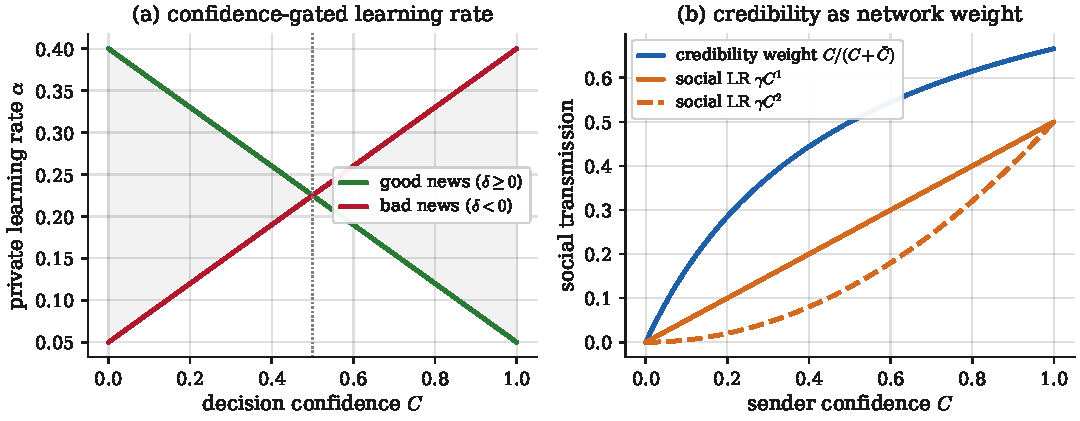
\includegraphics[width=0.82\textwidth]{fig_plasticity_quant.pdf}
\caption{Quantitative companion to Figure~\ref{fig:plasticity}. \textbf{(a)}~the
exact confidence-gated learning rates for good news ($\alpha_{\max}-(\alpha_{\max}-\alpha_{\min})C$)
and bad news ($\alpha_{\min}+(\alpha_{\max}-\alpha_{\min})C$), crossing at
$C=\tfrac12$. \textbf{(b)}~the credibility weight $C/(C+\bar C)$ and the social
learning rate $\gamma C^{\omega}$ ($\omega=1,2$) versus sender confidence.}
\label{fig:plasticityquant}
\end{figure}

\section{Robustness}
\label{app:robust}
We probe seven sensitivities (full CSVs in \texttt{paper/tables/};
Table~\ref{tab:robustness}, Figure~\ref{fig:robustness}). \textbf{R1} terminal
threshold $\{0.80,0.90,0.95\}$: dominant-regime area fractions are invariant.
\textbf{R2} horizon $T\in\{200,300,500,1000\}$: the unresolved region at
$\lambda\to0$ persists (genuine, not slow convergence); corrective and distortive
points are stable. \textbf{R3} early-lead strength $\delta$: a small lead
($\delta=0.04$) already triggers wrong consensus at the distortive point.
\textbf{R4} reward gap $|\Delta\mu|\in\{0.02,\dots,0.20\}$: wrong consensus
persists at the distortive point even for clearly distinguishable arms.
\textbf{R5} random graphs: balanced block, weighted stochastic-block and noisy
row-normalised $W$ give the same regimes, so the results do not depend on exact
quotient symmetry. \textbf{R6} phase-grid resolution $\{7^2,9^2,13^2\}$: the
area fractions are stable. \textbf{R7} reaction-time approximation: the
inverse-Gaussian and deterministic-mean reaction times give nearly identical
regime maps.

% Auto-generated -- robustness summary.
\begin{table}[t]\centering\small
\caption{Robustness summary (Appendix~\ref{app:robust}). Entries are the dominant-regime area fractions of the $(\lambda,\Gamma)$ plane, or P(wrong) at the operating point, as indicated. Full tables: \texttt{paper/tables/robustness\_*.csv}.}
\label{tab:robustness}
\begin{tabular}{lll}\toprule
Check & Variation & Result \\ \midrule
R1 threshold & $0.80/0.90/0.95$ & wrong-area $=0.53/0.53/0.53$ (invariant) \\
R2 horizon & $T=200\!-\!1000$ & near-zero stays unresolved; corrective/distortive stable \\
R3 initial lead & $\delta=0\!-\!0.16$ & P(wrong) $=0.12\!\to\!1.00$ (small lead suffices) \\
R4 reward gap & $|\Delta\mu|=0.02\!-\!0.20$ & P(wrong) $=1.00\!-\!1.00$ (persists) \\
R5 random graphs & balanced/SBM/noisy & distortive P(wrong) $=1.00/1.00/1.00$ \\
R6 grid resolution & $7^2/9^2/13^2$ & wrong-area $=0.49/0.53/0.51$ \\
R7 RT approximation & inverse-Gaussian vs.\ mean & wrong-area $=0.49$ vs.\ $0.49$ \\
\bottomrule\end{tabular}
\end{table}


\begin{figure}[t]
\centering
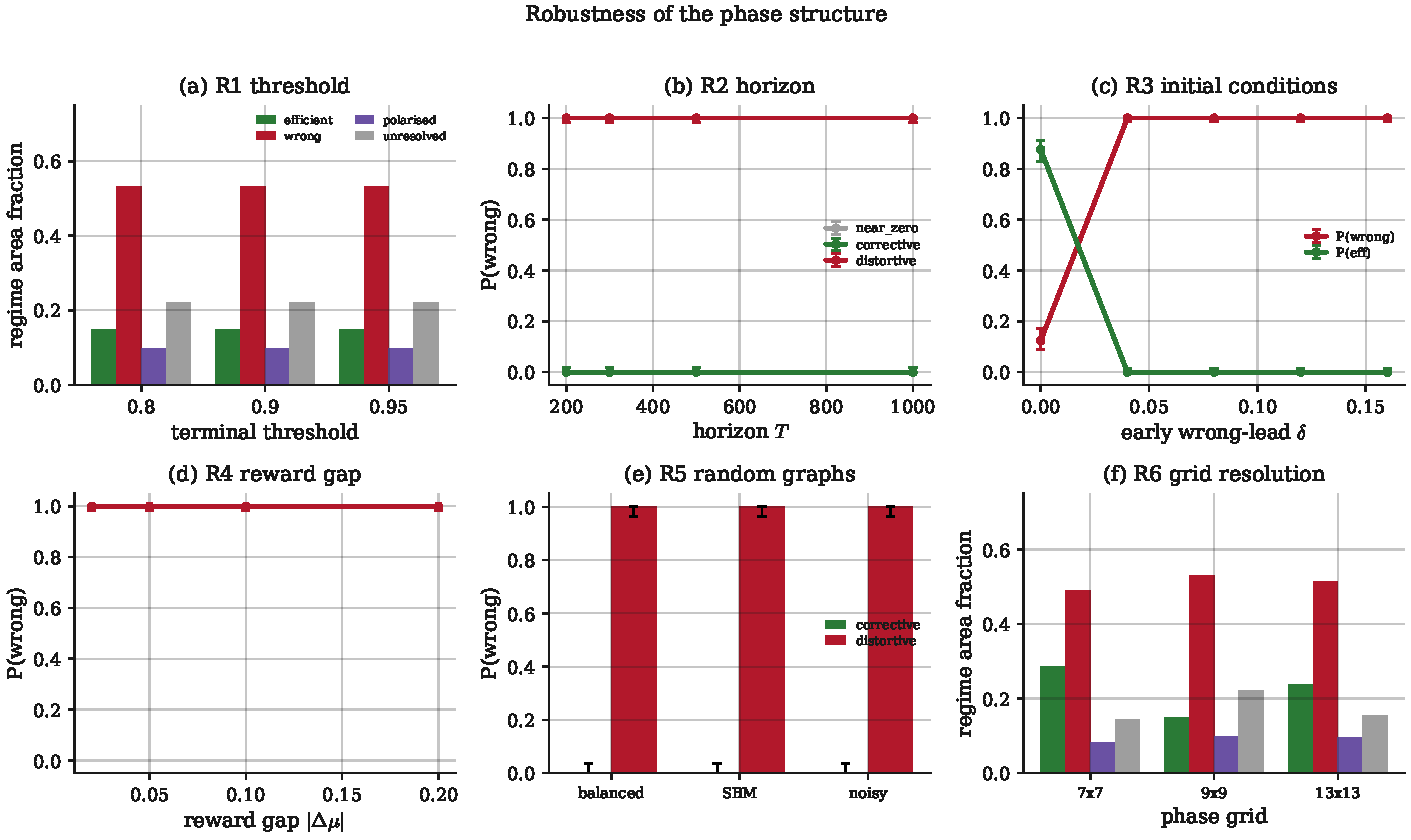
\includegraphics[width=\textwidth]{fig7_robustness.pdf}
\caption{Robustness of the phase structure. (a) regime area fractions are
invariant to the terminal threshold; (b) P(wrong) versus horizon for three
operating points; (c) P(wrong) and P(efficient) versus early-lead strength
$\delta$; (d) P(wrong) versus reward gap with Wilson intervals; (e) P(wrong)
under balanced, weighted-SBM and noisy graphs; (f) regime area fractions versus
phase-grid resolution. Full tables in Table~\ref{tab:robustness}.}
\label{fig:robustness}
\end{figure}

\section{Endogenous early-lead test of the amplification threshold}
\label{app:earlylead}
Proposition~\ref{prop:amplification} is a \emph{local} statement: it predicts when
small confidence-weighted mass gaps become self-amplifying, not the global regime
map. We test its predictive content without any imposed lead. Agents start from
neutral values ($Q=0.5$ on both arms) with a small reward gap
($\mu=0.53/0.47$) in two symmetric communities; a $25$-trial burn-in lets a
stochastic early asymmetry emerge, after which we measure the population
confidence-weighted mass gap and the terminal regime ($R=200$ per $\lambda$).
Figure~\ref{fig:earlylead} shows that wrong consensus is \emph{endogenous}: it is
essentially absent for $\lambda\lesssim\lambda^\star$ and rises as $\lambda$
crosses the analytical threshold $\lambda^\star\approx0.67$, while lock-in
fidelity is $\approx1$ --- the terminal consensus arm is the burn-in lead arm, so
the wrong-consensus replications are exactly those in which an early stochastic
gap formed toward the suboptimal arm and was amplified. The threshold therefore
predicts the onset of endogenous distortion, and the wrong-consensus regime does
not depend on a hand-picked initial condition.

\begin{figure}[ht]
\centering
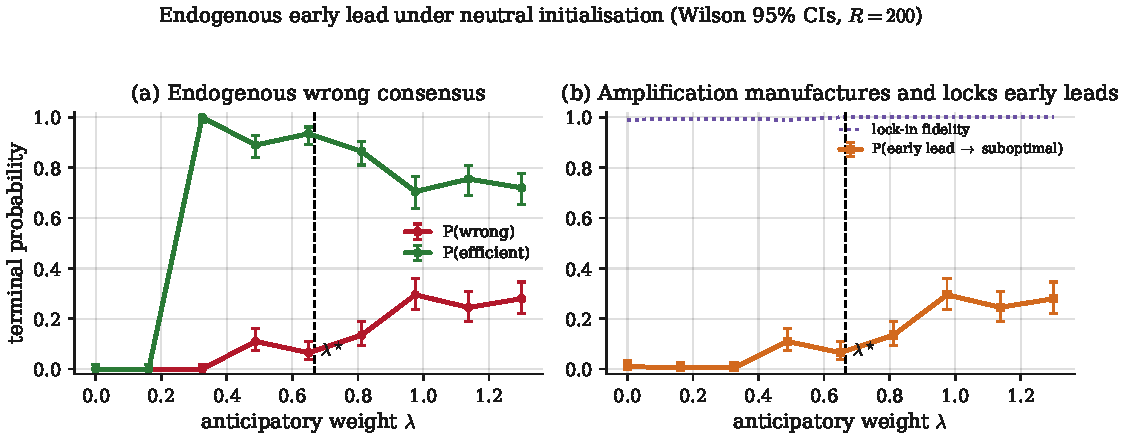
\includegraphics[width=\textwidth]{endogenous_early_lead.pdf}
\caption{Endogenous early lead (neutral initialisation, $R=200$ per $\lambda$).
(a) P(wrong) is $\approx0$ below the local amplification threshold
$\lambda^\star\approx0.67$ and rises above it, mirrored by a fall in
P(efficient). (b) the frequency of early suboptimal leads rises with $\lambda$
and they are locked in with fidelity $\approx1$. Data:
\texttt{tables/endogenous\_early\_lead.csv}.}
\label{fig:earlylead}
\end{figure}

\clearpage
\bibliographystyle{apalike}
\bibliography{endogenous_credibility}

\end{document}
